%\pdfoutput=1

\documentclass{l4proj}

%
% put any packages here
%

\usepackage{float}
\usepackage[labelfont=bf]{caption}

\usepackage{subfigure}

\usepackage{cleveref}

\usepackage[backend=bibtex,style=numeric]{biblatex}  %backend=biber is 'better'  

\usepackage[nottoc,notlot,notlof]{tocbibind}

\usepackage{pstricks, pst-node}

\setcounter{tocdepth}{3}
\usepackage{graphicx}
\usepackage{algorithmic}
\usepackage[ruled,vlined]{algorithm2e}
\usepackage{url}
\usepackage{alltt}
\urldef{\mailsa}\path|pat@dcs.gla.ac.uk|
\newcommand{\keywords}[1]{\par\addvspace\baselineskip
\noindent\keywordname\enspace\ignorespaces#1}
\newlength{\halftextwidth}
\setlength{\halftextwidth}{0.47\textwidth}

\usepackage{amsopn}
\DeclareMathOperator{\mod}{mod}

\newtheorem{theorem}{Theorem}
\newtheorem{definition}{Definition}


\renewcommand{\figurename}{Fig.}
\Crefformat{figure}{#2Fig.~#1#3}
\Crefmultiformat{figure}{Figs.~#2#1#3}{ and~#2#1#3}{, #2#1#3}{ and~#2#1#3}

\usepackage{listings}

\usepackage[thinlines]{easytable}

\usepackage{color, colortbl}
\definecolor{dkgreen}{rgb}{0,0.6,0}
\definecolor{gray}{rgb}{0.5,0.5,0.5}
\definecolor{mauve}{rgb}{0.58,0,0.82}

\lstset{
  %frame=tb,
  language=Java,
  %aboveskip=3mm,
  %belowskip=3mm,
  showstringspaces=false,
  columns=flexible,
  %basicstyle={\small\ttfamily},
  basicstyle=\scriptsize,     % the size of the fonts that are used for the code  
  numbers=left,
  stepnumber=1,
  numberstyle=\small\color{gray},    % the size of the fonts that are used for the line-numbers
  numbersep=10pt,             % how far the line-numbers are from the code
  keywordstyle=\color{blue},
  commentstyle=\color{dkgreen},
  stringstyle=\color{mauve},
  breaklines=true,            % sets automatic line breaking
  breakatwhitespace=false,    % sets if automatic breaks should only happen at whitespace
  showstringspaces=false,     % Don't show underscores as space characters
  %tabsize=4,
  frame=trBL,                 % adds a frame around the code
  frameround=fttt,
  captionpos=b,               % sets the caption-position to bottom
}

\RequirePackage{filecontents}
\begin{filecontents}{mybib.bib}
  @online{tarjanart,
  author = {Robert Tarjan},
  title = {HP Labs - Inventor interview - Robert Tarjan : The art of the algorithm},
  year = 2004,
  organization = {},
  file = {:./references/HP Labs - Inventor interview - Robert Tarjan : The art of the algorithm.html:html},
  url = {http://www.hpl.hp.com/news/2004/oct_dec/tarjan.html},
  urldate = {2016-03-14}
  }
  
@article{tarjan1972depth,
  title={Depth-first search and linear graph algorithms},
  author={Tarjan, Robert},
  journal={SIAM journal on computing},
  volume={1},
  number={2},
  pages={146--160},
  year={1972},
  publisher={SIAM}
}

@article{ford1956maximal,
  title={Maximal flow through a network},
  author={Ford, Lester R and Fulkerson, Delbert R},
  journal={Canadian journal of Mathematics},
  volume={8},
  number={3},
  pages={399--404},
  year={1956}
}

@inproceedings{regin1994filtering,
  title={A filtering algorithm for constraints of difference in CSPs},
  author={R{\'e}gin, Jean-Charles},
  booktitle={AAAI},
  volume={94},
  pages={362--367},
  year={1994}
}

@article{berge1957two,
  title={Two theorems in graph theory},
  author={Berge, Claude},
  journal={Proceedings of the National Academy of Sciences},
  volume={43},
  number={9},
  pages={842--844},
  year={1957},
  publisher={National Acad Sciences}
}

@article{haralick1980increasing,
  title={Increasing tree search efficiency for constraint satisfaction problems},
  author={Haralick, Robert M and Elliott, Gordon L},
  journal={Artificial intelligence},
  volume={14},
  number={3},
  pages={263--313},
  year={1980},
  publisher={Elsevier}
}

\end{filecontents}

\addbibresource{mybib.bib}

\begin{document}

\title{Animating a Sudoku solver}
\author{Gabriel I. Stratan}
\date{March 25, 2016}
\maketitle

\begin{abstract}
Sudoku is a popular puzzle played all over the world. It consists of filling in a 9x9 grid such that every row, column and 3x3 sub-grids have different digits from 1 to 9. Solving the puzzle will make use of the all-different algorithm from Constraint Programming for which an implementation will be provided. Finally, the program will animate all the steps done by the algorithm.
\end{abstract}

\educationalconsent
%
%NOTE: if you include the educationalconsent (above) and your project is graded an A then
%      it may be entered in the CS Hall of Fame
%
\tableofcontents
%==============================================================================
\chapter{Introduction}
\label{chap1intro}
\pagenumbering{arabic}

\noindent The Sudoku puzzle is a well known combinatorial problem where the goal is to fill in a partially completed 9x9 grid in such a way that a single digit cannot appear twice in the same row, column or 3x3 box. The problem is NP-complete and will be used as an example to introduce the concepts of the alldifferent algorithm used in Constraint Programming to solve many real-world combinatorial problems. Although the original 9x9 Sudoku puzzle can be solved in a fraction of a second using a variety of algorithms, the power and effectiveness of the algorithm introduced in this paper can be seen when trying to solve a 36x36 grid, where a solution is found in a matter or seconds, rather than days using a conventional approach. Students new to Constraint Programming will be shown a new way of approaching and solving real-world problems.

\section{Aims}
\noindent The aim of this project is to visualise how Constraint Programming techniques can be used to solve Sudoku puzzles. A Java application is developed to act as a teaching aid to be used by the lecturer to show students how the alldifferent algorithm works towards a solution. Sudoku puzzles represent an excellent choice to introduce the concept of the alldifferent constraint in a entertaining and engaging experience with the students. Students will be shown how to model the Sudoku puzzle as a Constraint Satisfaction Problem and get to the solution without resorting to guessing or bruteforcing. The constraint programming technique that will be used to solve the Sudoku puzzle is the same algorithm used worldwide to solve planning, scheduling, timetabling and supply chain management problems. The step by step visual representation of how the algorithm progresses towards a solution will help students better understand the new algorithm.

\section{Background}
The alldifferent algorithm introduced in 1994 by Jean-Charles Regin represents to this day a great achievemnt in Constraint Programming and other fields. 

\section{Motivation}
The motivation of this project is to provide a tool that makes it easier for a lecturer to introduce the alldifferent algorithm to its students by providing a step by step view of how the algorithm progresses. Students will find it easier to remember and undestand the algorithm through the use of the visualisations. The tool based on the Sudoku puzzle is a great way to visualize an important technique used to solve Constraint Satisfaction Problems and will provide an engaging learning experience to the students.

\section{Report Content}
The rest of the report will provide information on the algorithms used and their implementation in the project.
\begin{itemize}
\item Chapter~\ref{chap2background} covers details about the Sudoku puzzle and Constraint Programming.
\item Chapter~\ref{chap3alldiffconstraint} introduces a powerful constraint of difference.
\item Chapter~\ref{chap4alldiffalgos} explains the two algorithms needed to solve a constraint of difference.
\item Chapter~\ref{chap5alldiffdemo} covers a presentation of the project solving a Sudoku puzzle.
\item Chapter~\ref{chap6implementation} explains the implementation of the project.
\item Chapter~\ref{chap7conclusion} details the overall achievements of the project.
%appendices
\end{itemize}

\chapter{Background}
\label{chap2background}
\section{Sudoku}
\noindent Sudoku is a puzzle

\begin{figure}[H]
%\vspace{-6cm}
\begin{center}
%\hspace{-1.5cm}
\begin{minipage}{6cm}
%\centering
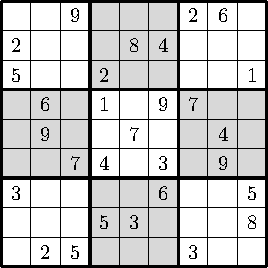
\includegraphics[height=6cm]{sudokugrid.pdf}
\caption{A Sudoku puzzle}
\label{sudokugrid1}
\end{minipage}
%\hfill
\hspace{2.5cm}
\begin{minipage}{6cm}
%\centering
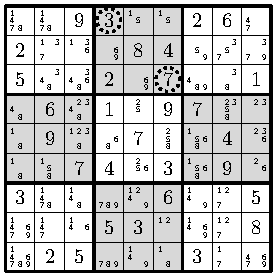
\includegraphics[trim=0.075cm 0.075cm 0.075cm 0.075cm, height=6cm]{sudokugrid2.pdf}
\caption{The state of the puzzle after the propagation}
\label{sudokugrid2}
\end{minipage}
\end{center}
\end{figure}

\section{Constraint Programming}
\noindent Constraint Programming (CP) is a technique originating from Artificial Intelligence used to solve hard real life combinatorial problems.

\noindent Constraints can be found everywhere in our daily life, and represent mathematical abstractions of the dependencies in the physical world. More formally, a constraint is a logical relationship among a number of variables, each with its own domain. The constraint therefore imposes restrictions on the values the variables can take. It is good to note that the values of the variables are not always numeric, a heterogeneous constraint would require a word (string) to have a specific length (numeric). The constraints are declarative as they only specify a relationship that must hold between variables and do not provide an algorithm to enforce the relationship.

\noindent Constraint Programming is the area of Computing Science that solves problems by specifying a list of constraints and then finding the solutions that satisfy all the constraints.
A Constraint Satisfaction Problem (CSP) can be defined as a triple $\mathcal{P} = <X, D, C>$, where $X$ represents a set of n variables $X = <x_1, x_2,..., x_n>$, $D$ represents the n domains associated to the n variables $D = <D_1, D_2,..., D_n>$ such that $x_i \in D_i$, and finally C represents a set of t constraints $C = <C_1, C_2,..., C_t>$. A constraint $C_i$ restricts the values one or more variables can simultaneously take.

\noindent A solution for a CSP $\mathcal{P}$ is a set of values $S = <s_1, s_2,..., s_n>$, such that each variable gets assigned a value from its domain and all the constraints are satisfied at once. The set of all the solutions to the problem is noted as $sol(\mathcal{P})$ for a CSP that has multiple solutions. One may also be interested in finding an optimal solution to the problem, one that for example minimizes the path of a traveling salesman. When $sol(\mathcal{P})$ is equal to the empty set, it means that the original CSP is unsatisfiable. This simple representation can be used to model complex real world problems such as planning, scheduling, timetabling, supply chain management and more.

\noindent There are two strategies for solving CSPs: inference and search. If all the variables in the problem have finite domains, this means the search space for a solution is finite and represented by all the possible combinations of the values of the variables. Although one can, in theory, enumerate all the possible combinations, we use inference and search to reduce the search space. Inference techniques remove large subspaces of the search tree through local constraint propagation on the basis that no solutions may be found using a particular value from the domain of a variable. Search techniques, such as backtracking, are used to systematically explore the search space, usually with the use of some heuristics, and reduce the search space whenever a single failure is found. Both strategies are frequently used together and work because a solution to a CSP must have all its constraints satisfied, therefore a local inconsistency on a subset of the variables will not result in a solution.

\noindent Backtracking search algorithms look for solutions to a CSP by traversing the search tree in a depth-first search manner. At each node of the search tree, a variable is assigned a value out of its domain, and the node gets extended with branches for the remaining values in the variable’s domain that need to be considered later, as they could be part of a solution. For example, consider a simple CSP problem with three variable $x$, $y$ and $z$. Suppose that the search algorithm already assigned a value to the variable $x$ out of its domain, and it reaches a node representing the variable $y$ with the domain $D_y = \{1, 2, 3\}$. The backtracking search algorithm will generate three branches, each one of them representing the variable $y$ getting instantiated to a value from its domain. For every value assigned to the variable $y$, all the constraints tied to this variable and the previously visited variables are checked to see if they still hold. When the constraints are not satisfied by a selected value for a variable, the algorithm proceeds in assigning and testing the rest of the values in the domain of $y$. Once all the values from the domain of the variable $y$ have been tried, the algorithm will backtrack to the previous variable, $x$ in this case, and assign it the next value from its domain. Note that every time backtracking occurs, subtrees of the search tree will no longer be generated and visited since they will not contain any solutions to the CSP. In the problem mentioned above, the subtree for the values of $z$ is no longer generated and tested as the partial solution made out of some specific values for $x$ and $y$ already violated the constraints of the problem. A complete solution is found once all the variables are assigned values that are allowed by the constraints. If the user is interested in only one solution to the problem, the search will terminate, otherwise the algorithm will continue to explore the search tree for other solutions. In the case the problem has no solutions, the algorithm will terminate after visiting all the possibilities in the search tree.

\noindent The efficiency of the backtracking search algorithm can be improved by performing constraint propagation to maintain consistency between the values of the variables and their associated constraints. Every time a variable is assigned a value from its domain, constraint propagation is made on the constraints the variable was part of. Propagation will check all the variables that were in a constraining relationship with the original variable and will remove values from their domain that are inconsistent with the problem requirements. By reducing the domains of the variables, the search tree is pruned and the efficiency of the search increases. The domain of a variable may be reduced to the empty set after propagation, which means that there is no value left for that variable that will satisfy the constraints and therefore backtracking should be initiated. On other occasions, the domain of a variable will be reduced to a single value, which means that the value for the variable is now known and removing the need to search through values that would not lead to a solution. The backtracking search algorithm will resume when the recursive propagation results in no changes to the domains of the variables. Information from constraint propagation is usually incorporated in the search algorithm in form of variable and value ordering heuristics that improve the efficiency of the search even more.

\noindent Variable and value ordering heuristics are ways to improve the backtracking search algorithm by prioritizing the instantiation of some variables and by choosing some values from their domain first. Ordering heuristics are essential to effectively solve hard combinatorial problems. The most popular heuristic is the fail-first approach, something Haralick and Elliot described as “To succeed, try first where you are most likely to fail.” \cite{haralick1980increasing}. The principle is to prioritize the instantiation of variables with the smallest domains of values. The assumption behind this is that branches in the search tree that have no solutions will be discovered earlier and pruned to bring a noticeable increase in efficiency later in the search. Consider the worst-case scenario when performing a backtracking search on a problem that has no solutions, the search tree will be much smaller as earlier failure is encouraged, making it faster to prove that a problem has no solutions. In the case of problems that start off with equally sized domains, the fail-first principle can still be applied by prioritizing the instantiation of the variables that take part in many constraints. Once a variable was selected for instantiation, some values from its domain could lead to a solution faster than others. The order values are chosen for assignment to the variables is only relevant when trying to find a single solution to the problem. The reason behind this is that trying to find all the solutions to a problem or proving that there are no solutions would have to traverse all the search space anyway. A heuristic to prioritize values from a domain is to assess the likelihood each value has in getting closer to a solution, a choice that will have minimum impact on the domain of other variables after propagation, therefore increasing the chances of finding a solution faster. 

\noindent Some solutions to a problem are better than others. Consider the Traveling Salesman Problem (TSP), where the shortest possible path between some cities should be found. The problem is NP-hard as the running time to find the solution increases exponentially with the number of cities. The general approach to the optimization problem is to introduce a constraint that minimizes a variable representing an objective, the length of the path in the case of the TSP. Finding an optimal solution is often hard, and proving optimality of a solution might be impossible for complex combinatorial problems.

\noindent Constraint Programming can be regarded as a form of declarative programming, where a user specifies a problem in terms of its variables, their domains and the constraints that should be satisfied. The computer then solves the given problem using a range of techniques that are general approaches to problem solving which can be applied to all the problems that can be modeled as constraint satisfaction problems.

\noindent The original exercise of finding an algorithm to solve a specific problem is now turned into an exercise of finding the best way to model the problem as a CSP, which can later be solved by the computer. The model can make the difference between efficient solving of a problem or a problem that cannot be solved due to its combinatorial complexity. There are usually many ways in which one can model the same problem, but the efficiency of the solution could be different. Consider a problem in which a number of $g$ guests should be offered a seat at one of the $t$ tables, with the constraint that couples should sit together. One could decide to represent each of the $g$ guests as a variable associated with an initial domain representing a listing of the $t$ tables, from which a choice for the table should be made based on the constraints. Another way to model the same problem is to have a number of $t$ variables representing the tables, each with an initial domain representing a listing of all the guests. The search for a solution would reduce the domains of the variables in both models until there is only a single table in the domains of the variables (for the first model where guests are variables), or in the case of the second model, until all the variables representing tables have the cardinality of their domains reduced to their sitting capacity. Although both models are logically equivalent, one may perform worse than the other because of how it’s represented in the memory of the computer.

\noindent When modeling a problem, it is important to avoid symmetries in the form of equivalent solutions. Symmetries represent waste computational resources during the backtracking search that is used to explore symmetrical assignments. One should avoid such symmetries by adding new constraints that will filter out the symmetrical solutions. Such constraints are problem specific. If it is necessary to find all the solutions to a problem, including the equivalent ones, one can easily perform permutations of the variables outside of the search space once the main solutions are found, thus avoiding exploring similar branches in the search tree. In the example problem mentioned above, there are symmetries in the solutions, as the same group of guests will be seated at different tables throughout the solutions. As we know tables are the same in real life and can be easily swapped without violating the constraints, such computations should not be made to improve efficiency of the search.

\noindent Real world problems are often large and over-constrained, which may raise difficulties in modeling them. Most of the time there are conflicting objectives such as trying to maximize the efficiency of a production facility, while minimizing the operational costs. Tradeoffs between the constraints should be made to come up with a solution to the problem. Problem decomposition should also used to break a large real world scenario into smaller problems that are easier to solve. Finally, one should consider which model is easier to upgrade when more constraints should be added.

\chapter{The Alldifferent Constraint}
\label{chap3alldiffconstraint}

\section{Review of Jean-Charles Regin's paper}
\noindent This section will introduce the reader to Jean-Charles Regin’s paper published in 1994, which describes a filtering algorithm for constraints of difference used in solving CSPs. As mentioned before, because the search for all the solutions to a CSP is NP-complete, there is a justified need to prune the search space before both before and during the search for the solutions.

\noindent A constraint of difference is defined as a relationship on a subset of the variables of a problem for which the values that are assigned to them should be all different. Many real world problems require such constraints. The paper starts by recognizing the need for a powerful n-ary constraint of difference, as binary constraint of difference cannot efficiently prune the search space of values for variables that will never be part of a solution, and for most instances it does not delete any value. Before the publishing of the paper, the common practice to represent n-ary constraint of difference was to model it as many binary constraints, one for each pair of variables in the n-ary constraint.

\noindent Consider a CSP problem with tree varibles $x$, $y$ and $z$ with their domains $D_x = \{1, 2\}$, $D_y = \{1, 2\}$ and $D_z = \{1, 2, 3\}$ with a constraint that solutions should have different values assigned to the variables. The first way one could model such a problem is by introducing 3 binary constraints of difference for all the pairs of the variables: $\{x, y\}$, $\{x, z\}$ and $\{y, z\}$. The second way, is to use a 3-ary constraint of difference between the variables $\{x, y, z\}$. The difference between the two approaches is that a propagation of the constraints for the binary representation will not reduce the domains of the variables. On the other hand, the model using a 3-ary constraint will successfully remove the value 1 and 2 from variable $z$, as they will already be used by $x$ and $y$.

\noindent Jean-Charles Regin goes on to describe a generalized constraint of difference to take advantage of the improved pruning of the search space. The aim is to achieve arc-consistency across all the variables in the CSP. A variable $x$ is said to be arc-consistent with the other variables participating in the same n-ary constraint if for all the values in $D_x$, there exists admissible values in the domains of the other variables such that the constraint holds. For the purpose of this exercise, the aim is to achieve diff-arc-consistency, which is concerned with achieving arc-consistency across the constraints of difference.

\noindent A constraint of difference $C$ can be represented by its value graph. The value graph of C is a bipartite graph where the variables in the constraint are grouped in the left partition of the graph, while the right partition represents a union of all the values from the domains of the variables. Edges between the two partitions of the graph connect the variables on the left hand side with values from their domains.

\noindent Matches in the value graph of $C$ are a subset of the edges in the graph, where no two edges share a common vertex. A maximum match is when all the vertices in the left partition have an edge to a vertex from the right partition, or more specifically, all the variables in the left partition are assigned a value from the right one.
After finding maximum matchings for all the value graphs associated to the constraints of difference in a given CSP, the values assigned to the variables do not break the diff-arc-consistency for the problem. Since each variable is assigned a value from its domain represented by an edge in the graph, and no two variables are assigned the same value, the diff-arc-consistency for the problem still holds. Knowing this property, an algorithm is built to filter the domains of the variables by removing values that would never be part of a maximum matching, therefore breaking the constraint and not leading to any solutions to the problem. It is good to note that by using the notation mentioned earlier, all the constraints of difference can be represented by their value graphs that have a space complexity in O(pd), where p is the arity of the constraint and d is the maximal cardinality of the domains for the variables in the constraint. Computing maximum matchings in a bipartite graph G = (X, Y, E) with m edges, can be done using Hopcroft and Karp’s (1973) algorithm which has a complexity of O(sqrt din modul de X... *m)TODO or Ford-Fulkerson (TODO) algorithm with a complexity O(VE). 

\noindent To begin reducing the domains of the variables, more definitions regarding matches are introduced. First, a vertex is $matched$ if there is an edge connecting it to a vertex in another partition of the graph. Vertices that are not matched are said to be $free$. Alternating paths represent paths made of edges that are alternatively matches and free and have a length corresponding to the number of edges in the path. Vital edges are edges that are part of all the maximum matchings in the value graph of a constraint.

\noindent Berge’s property (TODO) is used to find the edges that correspond to no maximum matchings and can therefore be deleted. According to the property, such edges are not vital and when starting from an arbitrary maximum matching, no even alternating paths can be found to include that edge. The algorithm starts by computing a maximum matching for the value graph of a constraint of difference. After this, an algorithm such as the one proposed by Tarjan (TODO) is used to find the strongly connected components in the graph. This means that edges in such a component will belong to even alternating paths, as the graph is bipartite and doesn’t have any odd cycles. The step of finding strongly connected components is necessary as this means that every edge connecting vertices from two strongly connected components can be deleted as it will never be part of an even alternating path. The deletion of an edge in the value graph of the constraint represents the reduction of a variable’s domain and is done for reasons independent from the constraint. The complexity of this algorithm proposed by Jean-Charles Regin’s is of $O(p^2 * d^2)$ for one constraint of difference.

\noindent Reducing the domain of a variable by deleting edges in the value graph of a constraint can trigger modifications for other constraints involving the same variable. If a variable is part of other constraints of difference, the author shows a more efficient propagation approach than simply repeating the same algorithm. The filtering algorithm for the second constraint builds on the information from the previous step by trying to remove the same edges in the value graph of the new constraint as long as they are not vital and a new maximum matching can be found.

\noindent The paper goes on to solve the zebra problem, a famous login puzzle. The author models the problem in different ways to prove that his approach can prune the search space of the problem more when compared to the previous methods used in the industry. One representation of the problem uses binary constraints for each pair of variables involved in the constraint of difference and another representation uses the n-ary constaint of difference introduced by the author. 

\noindent The results of his experiment show that the search space of the problem gets pruned more using the approach proposed in the paper, making the search for a solution to the problem more efficient. The same method was successfully used to solve the subgraph isomorphism problem. \cite{regin1994filtering}

\section{Usage example}
\noindent To demonstrate the usage and effects of the alldifferent constraint, we are going to use a simple example. The CSP problem will be modeled in Java and will make use of Choco3, a powerful free and open-source Java library used to solve Constraint Satisfaction Problems. The implamentation of the alldifferent constraint in the Choco3 library is based on Jean-Charles Regin's paper\cite{regin1994filtering} reviewed above.

\noindent The problem has three variables $x$, $y$, $z$ with the following initial domains: $x = \{1, 2\}$, $y = \{1, 2\}$ and $z = \{2, 3\}$. The constraint that should be satisfied by all the solutions of the problem is that $x$, $y$ and $z$ should all be different. The listing TODO shows how the problem is modeled and implemented using the Choco3 library.


\lstset{
  %frame=tb,
  language=Java,
  %aboveskip=3mm,
  %belowskip=3mm,
  columns=fullflexible,
  %basicstyle={\small\ttfamily},
  basicstyle=\small,     % the size of the fonts that are used for the code  
  numbers=left,
  stepnumber=1,
  numberstyle=\small\color{gray},    % the size of the fonts that are used for the line-numbers
  numbersep=10pt,             % how far the line-numbers are from the code
  keywordstyle=\color{blue},
  commentstyle=\color{dkgreen},
  stringstyle=\color{mauve},
  breaklines=true,            % sets automatic line breaking
  breakatwhitespace=false,    % sets if automatic breaks should only happen at whitespace
  showstringspaces=false,     % Don't show underscores as space characters
  %tabsize=4,
  frame=trBL,                 % adds a frame around the code
  frameround=fttt,
  captionpos=b,               % sets the caption-position to bottom
  showspaces=false,
}

\begin{figure}[H]
\lstset{caption={Usage of the alldifferent constraint in Choco3}, label=alldifferentChoco3}
%\lstinputlisting{AllDifferentExample.java}
\begin{lstlisting}
Solver solver = new Solver("AllDifferentExample");

IntVar x = VF.enumerated("x", new int[]{1, 2}, solver); 
IntVar y = VF.enumerated("y", new int[]{1, 2}, solver);
IntVar z = VF.enumerated("z", new int[]{2, 3}, solver);

solver.post(ICF.alldifferent(new IntVar[]{x, y, z}));

try{
    solver.propagate();
} catch (ContradictionException e){
    // Handle the exception
}

System.out.println(x + "\n" + y + "\n" + z);

if(solver.findSolution()){
    do{
	int x_val = x.getValue();
	int y_val = y.getValue();
	int z_val = z.getValue();

	System.out.println(x_val + "; " + y_val + "; " + z_val);
    } while(solver.nextSolution());
}
\end{lstlisting}
\end{figure}
 
\noindent Line 1 defines a Choco3 solver object, that will store the variables, their domains and constraints associated to them. Lines 3 to 5 define the three integer variables in the problem and their associated initial domains. The reference to the $solver$ object makes sure the variables are added to the model. Line 7 introduces the $alldifferent$ constraint between the three variables. The constraint is then posted to the model and the CSP is now fully modeled.

\noindent Before trying to find a solution, a call to the $propagate$ method is made on the model on line 10. The propagation algorithm will make all the constraints consistent by looping thorugh all the constraints in the model (only one in this case) with the aim of reducing the domains of the variables by removing values that will never part of a solution. When a value is removed from the domain of a variable, this might trigger a recursive propagation call on all its dependant variables to make the constraints consistent. The recursive propagation calls end when the problem is in a consistent state. It is good to note that propagation will preserve all the original solutions to the problem, while greatly reducing the search space.

\noindent The $ContradictionException$ on line 11 is an exception that is raised by Choco3 whenever a variable is left with an empty domain or is instantiated to a value that is out of its initial domain. This usually happens in overconstrained problems, where there are no values in the domains of the variables that satisfy all the constraints at once. In such cases, there would be no valid solutions to the problem. This is not the case with the example showcased here, as there are three variables with three different values in total.

\noindent Once the propagation is finished, a call is made on line 15 to output the updated domains of the variables. The updated domains after the call to the $propagation$ method are as follows: $x = \{1, 2\}$, $y = \{1, 2\}$ and $z = \{3\}$. The variable $z$ lost the value $2$ from its domain, while to the domains of $x$ and $y$ stayed the same. There are two reasons behind removing the value $2$ from the domain of variable $z$. Firstly, there would no solutions with $z$ taking the value of $2$ as this would leave either $x$ or $y$ with an empty domain after one of them takes the value of $1$. Secondly, two variables ($x$ and $y$) have the same domain of $\{1, 2\}$, therefore a solution that is consistent with the alldifferent constraint will have $x$ taking the value of $1$ and $y$ taking the value of $2$ (or vice-versa), making it impossible for $z$ to take the value of $2$.  Since we know that the values $1$ and $2$ will be attributed to $x$ and $y$, the value $2$ is removed from the domain of $z$ to reflect this change and reduce the search space.

\noindent Lines 17 to 25 will iterate over the two solutions of the problem and print the values for the variables. The solutions to the problem are $S_1 = \{1, 2, 3\}$ and $S_2 = \{2, 1, 3\}$ and they both contain values for the three variables that satisfy the alldifferent constraint.

\chapter{Algorithms for AllDiff}
\label{chap4alldiffalgos}

\section{Ford Fulkerson}
\noindent A flow represents a directed graph with special nodes called the source and the sink. Source nodes have outgoing edges to inner nodes, while sink nodes have incoming edges from inner nodes of the graph. The problem requires sending flows, for example water through a pipe, from the source to the sink, while conserving the equilibrium.

\noindent Flows need to get from the source to the sink by following the directed edges that often have different maximum capacity constraints, such as the diameter of a water pipe. Given a flow $f$ in graph $G$, we build a residual directed graph $G_f$. Forward edges in the graph haven’t reached their maximum capacity, while backward edges reached their upper bound. 

\noindent Ford-Fulkerson algorithm uses the residual graph to achieve a maximum flow in the graph. The algorithm looks for augmenting paths from source $S$ to sink $T$ in a breadth first-search manner. Once a path $p$ is found, we send the weight that will make the bottleneck edge in $p$ fill its maximum capacity. Then, we add (subtract) the weight of each forward (backward) edge in $p$. Forward edges that reach their maximum capacity turn into backward edges. This results in flow $f’$ that has a greater value than before. Berge’s theorem guarantees that once all the augmenting paths have been successively visited in the algorithm, the end result is a maximum flow of the graph \cite{berge1957two}.

\noindent The maximum matching problem is a special case of the maximum flow problem. For the purpose of our example, there will be only one source $S$ that has outgoing edges to the nodes in the left partition $L$ of the bipartite graph and one sink $T$ with incoming edges from the right partition $R$ of the graph. Nodes in $L$ are connected through edges to nodes in $R$. A matching TODO. A maximum matching TODO. To find a maximum matching for a Graph G, we add a source and sink nodes and set all edges to a maximum capacity of one. We then run the Ford-Fulkerson algorithm on the graph, by finding all the augmenting paths from free nodes in $L$ to free nodes in $R$.



\noindent Having a maximum matching for our graph, the next step in the alldifferent algorithm is to turn the previously undirected graph, into a directed one. The matches resulted from the Ford Fulkerson algorithm are assigned a direction from the 1 to 9 values to the corresponding cells of the Sudoku row. The edges that remain unused in the matching are given a direction from left to right (i.e. from the Sudoku cells of the row to the 1-9 values).

%graphffstart
\begin{figure}[H]
%graph1
  %\hfill
  \begin{minipage}{8.5cm}
    \centering
\psset{colsep=1.8cm,rowsep=0.5cm}
\begin{psmatrix}
[mnode=circle]a&1 \\
b&2 \\
c&3 \\
d&4 \\
e&5 \\
[mnode=none]L&[mnode=none]R 

\ncline[linewidth=2pt]{1,1}{1,2} % a > 1
\ncline{1,1}{2,2} % a > 2
\ncline{1,2}{2,1} % b > 1
\ncline{3,1}{2,2}  % c > 2
\ncline[linewidth=2pt]{3,1}{3,2} % c > 3 %TODO indent
\ncline{4,1}{3,2} % d > 3
\ncline[linewidth=2pt]{4,1}{4,2}  % d > 4
\ncline{4,1}{5,2} % d > 5
\ncline[linewidth=2pt]{5,2}{5,1} % e > 5

\end{psmatrix}
\caption{Initial graph}
\label{graph1}
\end{minipage}
%graph2
\hfill
\begin{minipage}{8.5cm}
\centering
  \psset{colsep=2.0cm,rowsep=0.5cm, arrows=->, arrowsize=6pt, arrowinset=0, labelsep=3pt}
\begin{psmatrix}
&[mnode=circle]a&[mnode=circle]1 \\
&[mnode=circle]b&[mnode=circle]2 \\
[mnode=circle]S&[mnode=circle]c&[mnode=circle]3&[mnode=circle]T\\
&[mnode=circle]d&[mnode=circle]4 \\
&[mnode=circle]e&[mnode=circle]5 \\
[mnode=none]&L&R

\ncline[linecolor=blue]{3,1}{1,2}\mput*{0/1}
\ncline[linecolor=blue]{3,1}{2,2}\mput*{0/1}
\ncline[linecolor=blue]{3,1}{3,2}\mput*{0/1}
\ncline[linecolor=blue]{3,1}{4,2}\mput*{0/1}
\ncline[linecolor=blue]{3,1}{5,2}\mput*{0/1}

\ncline{1,2}{1,3}\mput*{0/1} % a > 1
\ncline{1,2}{2,3}\mput*{0/1} % a > 2
\ncline{2,2}{1,3}\mput*{0/1} % b > 1
\ncline{3,2}{2,3}\mput*{0/1} % c > 2
\ncline{3,2}{3,3}\mput*{0/1} % c > 3
\ncline{4,2}{3,3}\mput*{0/1} % d > 3
\ncline{4,2}{4,3}\mput*{0/1} % d > 4
\ncline{4,2}{5,3}\mput*{0/1} % d > 5
\ncline{5,2}{5,3}\mput*{0/1} % e > 5

\ncline[linecolor=blue]{1,3}{3,4}\mput*{0/1}
\ncline[linecolor=blue]{2,3}{3,4}\mput*{0/1}
\ncline[linecolor=blue]{3,3}{3,4}\mput*{0/1}
\ncline[linecolor=blue]{4,3}{3,4}\mput*{0/1}
\ncline[linecolor=blue]{5,3}{3,4}\mput*{0/1}
\end{psmatrix}
\caption{S\&T nodes added}
\label{graph2}
\end{minipage}
\vspace*{1cm}
%graph3
%\hfill
%\caption{Title for both}
%\end{figure}

%\begin{figure}[h]
%\hfill
\begin{minipage}{8.5cm}
  \centering
\psset{colsep=2.0cm,rowsep=0.5cm, arrows=->, arrowsize=6pt, arrowinset=0, labelsep=3pt}
\begin{psmatrix}
&[mnode=circle]a&[mnode=circle]1 \\
&[mnode=circle]b&[mnode=circle]2 \\
[mnode=circle]S&[mnode=circle]c&[mnode=circle]3&[mnode=circle]T\\
&[mnode=circle]d&[mnode=circle]4 \\
&[mnode=circle]e&[mnode=circle]5 \\
[mnode=none]&L&R

\ncline[linewidth=2pt, linecolor=red]{1,2}{3,1}\mput*{1/1} 
\ncline{3,1}{2,2}\mput*{0/1}
\ncline[linewidth=2pt, linecolor=red]{3,2}{3,1}\mput*{1/1}
\ncline[linewidth=2pt, linecolor=red]{4,2}{3,1}\mput*{1/1}
\ncline[linewidth=2pt, linecolor=red]{5,2}{3,1}\mput*{1/1}

\ncline[linewidth=2pt, linecolor=red]{1,3}{1,2}\mput*{1/1} % a > 1
\ncline{1,2}{2,3}\mput*{0/1} % a > 2
\ncline{2,2}{1,3}\mput*{0/1} % b > 1
\ncline[linewidth=2pt, linecolor=red]{2,3}{3,2}\mput*{1/1} % c > 2
\ncline{3,2}{3,3}\mput*{0/1} % c > 3
\ncline[linewidth=2pt, linecolor=red]{3,3}{4,2}\mput*{1/1} % d > 3
\ncline{4,2}{4,3}\mput*{0/1} % d > 4
\ncline{4,2}{5,3}\mput*{0/1} % d > 5
\ncline[linewidth=2pt, linecolor=red]{5,3}{5,2}\mput*{1/1} % e > 5

\ncline[linewidth=2pt, linecolor=red]{3,4}{1,3}\mput*{1/1}
\ncline[linewidth=2pt, linecolor=red]{3,4}{2,3}\mput*{1/1}
\ncline[linewidth=2pt, linecolor=red]{3,4}{3,3}\mput*{1/1}
\ncline{4,3}{3,4}\mput*{0/1}
\ncline[linewidth=2pt, linecolor=red]{3,4}{5,3}\mput*{1/1}
\end{psmatrix}
\caption{Greedy match}
\label{graph3}
\end{minipage}
%graph4
\hfill
\begin{minipage}{8.5cm}
\centering
  \psset{colsep=2.0cm,rowsep=0.5cm, arrows=->, arrowsize=6pt, arrowinset=0, labelsep=3pt}
\begin{psmatrix}
&[mnode=circle]a&[mnode=circle]1 \\
&[mnode=circle]b&[mnode=circle]2 \\
[mnode=circle]S&[mnode=circle]c&[mnode=circle]3&[mnode=circle]T\\
&[mnode=circle]d&[mnode=circle]4 \\
&[mnode=circle]e&[mnode=circle]5 \\
[mnode=none]&L&R

\ncline[linewidth=2pt]{1,2}{3,1}\mput*{1/1}
\ncline[linewidth=2pt, linecolor=green]{3,1}{2,2}\mput*{0/1}
\ncline[linewidth=2pt]{3,2}{3,1}\mput*{1/1}
\ncline[linewidth=2pt]{4,2}{3,1}\mput*{1/1}
\ncline[linewidth=2pt]{5,2}{3,1}\mput*{1/1}

\ncline[linewidth=2pt, linecolor=red]{1,3}{1,2}\mput*{1/1} % a > 1
\ncline[linewidth=2pt, linecolor=green]{1,2}{2,3}\mput*{0/1} % a > 2
\ncline[linewidth=2pt, linecolor=green]{2,2}{1,3}\mput*{0/1} % b > 1
\ncline[linewidth=2pt, linecolor=red]{2,3}{3,2}\mput*{1/1} % c > 2
\ncline[linewidth=2pt, linecolor=green]{3,2}{3,3}\mput*{0/1} % c > 3
\ncline[linewidth=2pt, linecolor=red]{3,3}{4,2}\mput*{1/1} % d > 3
\ncline[linewidth=2pt, linecolor=green]{4,2}{4,3}\mput*{0/1} % d > 4
\ncline{4,2}{5,3}\mput*{0/1} % d > 5
\ncline[linewidth=2pt]{5,3}{5,2}\mput*{1/1} % e > 5

\ncline[linewidth=2pt]{3,4}{1,3}\mput*{1/1}
\ncline[linewidth=2pt]{3,4}{2,3}\mput*{1/1}
\ncline[linewidth=2pt]{3,4}{3,3}\mput*{1/1}
\ncline[linewidth=2pt, linecolor=green]{4,3}{3,4}\mput*{0/1}
\ncline[linewidth=2pt]{3,4}{5,3}\mput*{1/1}
\end{psmatrix}
\caption{Longer augmenting path}
\label{graph4}
\end{minipage}

\vspace*{1cm}
%\null\hfill
%graph5
\begin{minipage}{8.5cm}
  \centering
\psset{colsep=2.0cm,rowsep=0.5cm, arrows=->, arrowsize=6pt, arrowinset=0, labelsep=3pt}
\begin{psmatrix}
&[mnode=circle]a&[mnode=circle]1 \\
&[mnode=circle]b&[mnode=circle]2 \\
[mnode=circle]S&[mnode=circle]c&[mnode=circle]3&[mnode=circle]T\\
&[mnode=circle]d&[mnode=circle]4 \\
&[mnode=circle]e&[mnode=circle]5 \\
[mnode=none]&L&R

\ncline[linewidth=2pt]{1,2}{3,1}\mput*{1/1}
\ncline[linewidth=2pt]{2,2}{3,1}\mput*{1/1}
\ncline[linewidth=2pt]{3,2}{3,1}\mput*{1/1}
\ncline[linewidth=2pt]{4,2}{3,1}\mput*{1/1}
\ncline[linewidth=2pt]{5,2}{3,1}\mput*{1/1}

\ncline{1,2}{1,3}\mput*{0/1} % a > 1
\ncline[linewidth=2pt]{2,3}{1,2}\mput*{1/1} % a > 2
\ncline[linewidth=2pt]{1,3}{2,2}\mput*{1/1} % b > 1
\ncline{3,2}{2,3}\mput*{0/1} % c > 2
\ncline[linewidth=2pt]{3,3}{3,2}\mput*{1/1} % c > 3
\ncline{4,2}{3,3}\mput*{0/1} % d > 3
\ncline[linewidth=2pt]{4,3}{4,2}\mput*{1/1} % d > 4
\ncline{4,2}{5,3}\mput*{0/1} % d > 5
\ncline[linewidth=2pt]{5,3}{5,2}\mput*{1/1} % e > 5

\ncline[linewidth=2pt]{3,4}{1,3}\mput*{1/1}
\ncline[linewidth=2pt]{3,4}{2,3}\mput*{1/1}
\ncline[linewidth=2pt]{3,4}{3,3}\mput*{1/1}
\ncline[linewidth=2pt]{3,4}{4,3}\mput*{1/1}
\ncline[linewidth=2pt]{3,4}{5,3}\mput*{1/1}
\end{psmatrix}
\caption{New matching}
\label{graph5}
\end{minipage}
\hfill
%graph6
\begin{minipage}{8.5cm}
\centering
  \psset{colsep=2.0cm,rowsep=0.5cm}
\begin{psmatrix}
[mnode=circle]a&1 \\
b&2 \\
c&3 \\
d&4 \\
e&5 \\
[mnode=none]L&[mnode=none]R 

\ncline{1,1}{1,2}% a > 1
\ncline[linewidth=2pt]{1,1}{2,2}% a > 2
\ncline[linewidth=2pt]{1,2}{2,1}% b > 1
\ncline{3,1}{2,2}  % c > 2
\ncline[linewidth=2pt]{3,1}{3,2} % c > 3
\ncline{4,1}{3,2} % d > 3
\ncline[linewidth=2pt]{4,1}{4,2}  % d > 4
\ncline{4,1}{5,2} % d > 5
\ncline[linewidth=2pt]{5,2}{5,1} % e > 5
\end{psmatrix}
\caption{Maximum matching}
\label{graph6}
\end{minipage}
%\null\hfill
\caption{Ford–Fulkerson algorithm}
\label{fig:ff_1_6}
\end{figure}
%graphffend

% use \mathit to fix italics spacing
\begin{algorithm}[H]
\DontPrintSemicolon
\nl $\textbf{void} ~FordFulkerson(\textbf{Graph}~G)$ \;
\nl \Begin{
\nl $\textbf{Global} ~ \textbf{int} ~ capacity[][] \gets getCapacity(G)$ \;
\nl $\textbf{Global} ~ \textbf{int} ~ n \gets |V(G)|$ \;
\nl $\textbf{Global} ~ \textbf{int} ~ source \gets 0$ \;
\nl $\textbf{Global} ~ \textbf{int} ~ sink \gets n-1$ \;
\nl $\textbf{Global} ~ pred \gets ~new~\textbf{int}[n]$ \;
\nl $\textbf{Global} ~ visited \gets ~new~\textbf{boolean}[n]$ \;
\nl $\textbf{Global} ~ Q \gets ~new~\textbf{Queue}()$ \;
\nl \While {$\mathit{bfs}(G)$}{
\nl $update()$ \;
}

} %begin FordFulkerson

\;
\nl $\textbf{boolean} ~\mathit{bfs}(\textbf{Graph} ~ G)$ \;
\nl \Begin{
\nl $clear(Q) $ \;
\nl $fill(pred, -1) $ \;
\nl $fill(visited, false) $ \;
\nl $enqueue(source, Q) $ \;
\nl $visited[source] \gets ~true $\;
\nl \While {$(\neg isEmpty(Q))$}{
\nl $\textbf{int} ~ v \gets dequeue(Q) $ \;
\nl \lIf {$v = ~ sink $}{ $\textbf{return} ~ true $ }

\nl \For {$w \gets ~ 0 ~ to ~ n $}{
\nl \If {$\neg visited[w] ~ \textbf{and} ~ capacity[v][w] > 0$}{ 
\nl $ pred[w] \gets v$ \;
\nl $ enqueue(w, Q)$ \;
\nl $ visited[w] \gets true$ \;
} %if
} %for
} %while
\nl $\textbf{return} ~ \mathit{false} $ \;
} %begin bfs

\;

\nl $\textbf{void} ~update()$ \;
\nl \Begin{

\nl $\textbf{int} ~ f \gets minCost()$ \;
\nl $\textbf{int} ~ v \gets sink $ \;

\nl \While {$pred[v] \neq -1$}{
\nl $\textbf{int} ~ u \gets pred[v] $ \;
\nl $capacity[u][v] \gets capacity[u][v] - f $ \;
\nl $capacity[v][u] \gets capacity[v][u] + f $ \;
\nl $v \gets u$ \;
} %while

} %begin updateR

\;

\nl $\textbf{int} ~minCost()$ \;
\nl \Begin{

\nl $\textbf{int} ~ minCost \gets \infty $ \;
\nl $\textbf{int} ~ v \gets sink $ \;

\nl \While {$pred[v] \neq -1$}{
\nl $minCost \gets minimum(minCost, capacity[pred[v]][v])$ \;
\nl $v \gets pred[v]$ \;
}
\nl $\textbf{return} ~ minCost$ \;
} %begin updateR

\caption{Ford Fulkerson}
\label{FordFulkersonPC}
\end{algorithm}

\noindent Ford Fulkerson's algorithm for finding a maximum flow in a graph is shown in algorithm \ref{FordFulkersonPC}. \cite{ford1956maximal}. The $Ford$ $Fulkerson$ procedure on line 1 takes a graph $G$ as an argument and represents the start of the algorithm. The graph passed as an argument holds information about the capacity of each edge. Line 3 stores the capacity of the graph $G$ in a global two-dimensional integer array. The capacity of an edge between vertices $u$, $v$ is stored in $capacity[u][v]$. Line 4 declares an integer $n$ used to store the number of vertices in the given graph. Lines 5 and 6 declare two integers called $source$ and $sink$ representing references to the first and the last vertices in the given graph.

\noindent In line 7 we declare a vertex-indexed array $pred$ that is used to store references to the previous vertex discovered in the breadth-first search tree. Line 8 declares a vertex-indexed array $visited$ used to keep track if a vertex has already been visited in the breadth-first search procedure. Line 9 declares a queue of integers $Q$ used to store vertices in the order they are visited.

\noindent The algorithm consists of repeated calls to the breadth-first search procedure (line 10). In line 11, we call the update procedure to update the capacities of the edges after finding augmenting paths.

\noindent The $breadth\textit{-}first ~ search$ procedure starts at line 12 and takes a graph $G$ as an argument. In lines 14 to 16, the queue $Q$, $pred$ and $visited$ array are reset to have default values. The breadth-first search calls always start from the first vertex, representing the source. This vertex is enqueued on queue $Q$ in line 17 and is marked as visited in line 18.

\noindent Lines 19 to 26 contain a loop performing changes on the queue $Q$ that is used to store an augmenting path. The loop starts on line 20 by dequeuing a vertex from the queue $Q$ and storing it in $v$. Line 21 forces the breadth-first search procedure to return $true$ when we reach the last vertex in the graph, the sink. Lines 22 to 26 contain a loop over all the vertices $w$ in the graph. In line 23 we check to see if the discovered vertex $w$ hasn't been already visited and we consider it if it still has available capacity. Line 24 stores the index value of $w$'s predecessor in the augmenting path. Line 25 enqueues the discovered vertex $w$ on the queue $Q$ and marks it as visited in line 26. Finally, the breadth-first search procedure returns $false$ when no more augmenting paths are found.

\noindent The $update$ procedure at line 28 is used to update the capacities of the edges in the graph to reflect the updated flow. Line 30 declares an integer $f$ used to store the amount of flow we are adding along the found path. The value for $f$ is calculated in the $minCost$ procedure at line 37. Line 31 declares an integer $v$, initially representing the sink which is the last vertex in the graph. Lines 32 to 35 contain a loop that updates the capacities of the edges in the augmenting path. Line 33 uses the integer $u$ to store the index of a vertex that is the predecessor of vertex $v$ along the path. Lines 34 and 35 updates the flow along the edge from $u$ to $v$ and $v$ to $u$ by the found difference. Finally, $v$ is updated on line 36 to take the value of $u$ such that the while loop continues to change the capacities of the remaining edges along the path.

\noindent The $minCost$ procedure at line 37 is used to find the amount of flow to be sent along the new augmenting path from the sink to the source. The value is equal to the minimum capacity that is still available along the edges of the path. Line 39 declares an integer $minCost$ used to represent the current value of the minimum cost, initialized to a big value. Line 40 declares an integer variable $v$ initially used to store a reference to the sink vertex. Lines 41 to 43 contain a loop over the edges along the path, starting from the sink toward the source. Line 42 updates the value of $minCost$ if the current edge in the loop has a smaller capacity left than what was previously discovered. The $minimum$ procedure returns the minimum of two given integers. Line 43 updates the value of integer $v$ to its predecessor so the loop can continue along the path until it reaches the $source$. At the end of the $minCost$ procedure, we return the value of the currently found $minCost$ variable.

\newpage

\section{Tarjan algorithm}
\noindent A strongly connected component $SCC$ of a directed graph $G$ is a maximal set of vertices such that every vertex is reachable from every other vertex by following the directed edges.

\noindent There are four kinds of edges in a depth-first traversal: tree edges, forward edges, back edges and cross edges. Tree edges are edges between a vertex and vertices that were not previously visited. Forward edges are from ancestor vertices to descendant vertices that were already visited during the search. Back edges link descendant vertices back to already visited ancestor vertices. Lastly, cross edges represent edges between two vertices that are neither an ancestor nor a descendant for each other, such as the edges between different components of the graph. 

\noindent For each vertex in a graph G, the algorithm keeps track of two properties. The first property we remember is the $index$ of the node, its consecutive order of discovery during the depth-first search, a value that will remain constant throughout the algorithm. The second property associated with all the nodes is named $low$ and keeps track of the lowest (oldest) ancestor reachable from their position in the graph. As each node of the graph gets discovered in a depth-first search manner, the initial value that $low$ gets assigned is the same as the $order$ the node was discovered. The value for $low$ may get changed during the search if an ancestor for the node is discovered by following a back edge. After the recursive depth-first search finishes visiting all of a node’s neighbours, the node’s value for $low$ gets updated to the lowest index of its oldest reachable ancestor. If the value for $low$ of a node stays the same even after visiting all of its neighbours, then it means it is the root of a strongly connected component or it’s an individual vertex that will be a component on its own. \cite{tarjan1972depth}

\noindent For the purpose of finding SCCs, every time a node is discovered in the search, the node is put on a stack $S$. After returning from the recursive DFS calls on all of the adjacent neighbours of vertex, if both $index$ and $low$ have the same value, it means we’ve finished discovering a SCC. The vertices in the newly discovered strongly connected component will be popped from the stack $S$ until we reach the current vertex representing the root of the SCC. Vertices that are part of other SCCs are still left on the stack as they have different roots represented by the value of $low$.

\noindent Figure 2.8  TODO shows a bipartite directed graph with 18 vertices. There are 9 backward edges that represent the maximum matching found using the Ford-Fulkerson algorithm in section TODO. The rest of the possible edges are assigned a forward direction. This graph is similar to the graphs that will be generated to represent a row, column or one of the nine sub-grids of the Sudoku puzzle. For example, the left partition of the graph will contain the nine variables of a Sudoku row, and the right partition will contain the digits from 1 to 9. The edges will then link each variable of the row to values that are still available in their domain.

\noindent The Table 2.1 TODO contains the output after running the Tarjan’s algorithm on the graph in figure 2.8 TODO. As previously discussed, vertices are visited in a depth-first search manner, in this case starting from the first vertex. Each node has two properties associated to it: its order of discovery or $inded$, and its oldest reachable ancestor. Initially, both properties take the value of the index, but as the algorithm progresses the values for low may become lower after visiting all of the neighbours of the node and finding the oldest (lowest) reachable ancestor. All vertices are pushed on a stack in the order they are visited. Once a back edge is found in the graph, vertices that are currently on the stack get popped including the root of the newly discovered SCC. Note that vertices may still remain on the stack as they will be part of different components that have other roots. As each vertex is made part of a component, its value for $low$ gets updated to a large value to mark it as already part of a component such that it will not become the root of another component in the future.

\noindent The graph in figure 2.9 TODO shows the 5 strongly connected components identified after running Tarjan’s algorithm on the initial graph in figure 2.8 TODO. Vertices that have the same background are part of the same component; meaning that one vertex can reach every other vertex in the component by following the directed edges. Note that some vertices make a component on their own as there is no way to reach them again in a cycle.

\iffalse ///////////////////////////
Now that all the edges from the graph are directed, the next step in the alldifferent algorithm is to find the strongly connected components of the graph. In order to do this, we introduce now Tarjan’s algorithm for finding strongly connected components  (SCCs) in a given graph G.

\noindent The algorithm starts by visiting every node in the directed graph in a depth first search manner. During the search, nodes are added to a stack in the order they are discovered only if they were not already part of the stack. 

\noindent Backtracking is triggered when we reach a node that is upper compared to our previous node (if(min < low[u])).  We know this by keeping record of the upmost node reachable from node u, including node u itself during each branch of the depth first search. We use low to denote the minimum index representing the upmost node in the branch.

\noindent If the current node is less than the upper node is less than the current index, it means that we have 

\noindent If the upper node is equal to the node we are currently visiting, then the algorithm just found a strongly connected component that contains all nodes on the stack starting from the top of it, until encountering the current node. The nodes are popped out of the stack and a SCC id/index is assigned to it for later use. Once the current node is reached, we increment the count of the SCCs to start filling a new SCC.

\noindent // write that there are no self loops / self edges (u!=i)

 /////////////////////////////////////////////////////
\fi

\newpage

%graphtstart
\begin{figure}[H]
%graph21
\begin{minipage}{8.0cm}
\centering
\psset{colsep=6cm, rowsep=0.3cm, arrows=->, arrowsize=6pt, arrowinset=0, radius=3cm}
\begin{psmatrix}
[mnode=circle]1&10 \\
2&11 \\
3&12 \\
4&13 \\
5&14 \\
6&15 \\
7&16 \\
8&17 \\
9&18 \\
[mnode=none]L&[mnode=none]R 

\nccurve[angleA=180, offsetA=3pt, offsetB=3pt, linewidth=2pt]{1,2}{1,1} % a > 1 X
\nccurve[angleB=180, offsetA=3pt, offsetB=3pt]{1,1}{8,2} % a > 8

\nccurve[angleB=180, offsetA=3pt, offsetB=3pt]{2,1}{2,2} % b > 2
\nccurve[angleA=180, offsetA=3pt, offsetB=3pt, linewidth=2pt]{3,2}{2,1} % b > 3 X

\nccurve[angleA=180, offsetA=3pt, offsetB=3pt, linewidth=2pt]{2,2}{3,1} % c > 2 X
\nccurve[angleB=180, offsetA=3pt, offsetB=3pt]{3,1}{3,2} % c > 3

\nccurve[angleB=180, offsetA=3pt, offsetB=3pt]{4,1}{2,2} % d > 2 
\nccurve[angleA=180, offsetA=3pt, offsetB=3pt, linewidth=2pt]{4,2}{4,1} % d > 4 X
\nccurve[angleB=180, offsetA=3pt, offsetB=3pt]{4,1}{5,2} % d > 5

\nccurve[angleB=180, offsetA=3pt, offsetB=3pt]{5,1}{4,2} % e > 4 
\nccurve[angleB=180, offsetA=3pt, offsetB=3pt]{5,1}{5,2} % e > 5
\nccurve[angleA=180, offsetA=3pt, offsetB=3pt, linewidth=2pt]{6,2}{5,1} % e > 6 X

\nccurve[angleB=180, offsetA=3pt, offsetB=3pt]{6,1}{4,2} % f > 4
\nccurve[angleA=180, offsetA=3pt, offsetB=3pt, linewidth=2pt]{5,2}{6,1} % f > 5 X
\nccurve[angleB=180, offsetA=3pt, offsetB=3pt]{6,1}{6,2} % f > 6

\nccurve[angleB=180, offsetA=3pt, offsetB=3pt]{7,1}{2,2} % g > 2
\nccurve[angleA=180, offsetA=3pt, offsetB=3pt, linewidth=2pt]{7,2}{7,1} % g > 7 X
\nccurve[angleB=180, offsetA=3pt, offsetB=3pt]{7,1}{9,2} % g > 9

\nccurve[angleB=180, offsetA=3pt, offsetB=3pt]{8,1}{3,2} % h > 3
\nccurve[angleB=180, offsetA=3pt, offsetB=3pt]{8,1}{7,2} % h > 7
\nccurve[angleA=180, offsetA=3pt, offsetB=3pt, linewidth=2pt]{8,2}{8,1} % h > 8 X

\nccurve[angleB=180, offsetA=3pt, offsetB=3pt]{9,1}{2,2} % i > 2
\nccurve[angleB=180, offsetA=3pt, offsetB=3pt]{9,1}{3,2} % i > 3
\nccurve[angleB=180, offsetA=3pt, offsetB=3pt]{9,1}{5,2} % i > 5
\nccurve[angleB=180, offsetA=3pt, offsetB=3pt]{9,1}{8,2} % i > 8
\nccurve[angleA=180, offsetA=3pt, offsetB=3pt, linewidth=2pt]{9,2}{9,1} % i > 9 X

\end{psmatrix}
\caption{Initial graph}
\label{graph21}
\end{minipage}
%graph22
\hfill
\begin{minipage}{8.0cm}
\centering
\definecolor{applegreen}{rgb}{0.55, 0.71, 0.0}
\definecolor{amber}{rgb}{1.0, 0.75, 0.0}
\definecolor{babyblue}{rgb}{0.54, 0.81, 0.94}
\definecolor{americanrose}{rgb}{1.0, 0.01, 0.24}
%yellow

\psset{colsep=6cm, rowsep=0.3cm, arrows=->, arrowsize=6pt, arrowinset=0, radius=3cm}
\begin{psmatrix}
[mnode=circle][fillstyle=solid,fillcolor=babyblue]1&[fillstyle=solid,fillcolor=americanrose]10 \\
[fillstyle=solid,fillcolor=amber]2&[fillstyle=solid,fillcolor=amber]11 \\
[fillstyle=solid,fillcolor=amber]3&[fillstyle=solid,fillcolor=amber]12 \\
[fillstyle=solid,fillcolor=applegreen]4&[fillstyle=solid,fillcolor=applegreen]13 \\
[fillstyle=solid,fillcolor=applegreen]5&[fillstyle=solid,fillcolor=applegreen]14 \\
[fillstyle=solid,fillcolor=applegreen]6&[fillstyle=solid,fillcolor=applegreen]15 \\
[fillstyle=solid,fillcolor=yellow]7&[fillstyle=solid,fillcolor=yellow]16 \\
[fillstyle=solid,fillcolor=yellow]8&[fillstyle=solid,fillcolor=yellow]17 \\
[fillstyle=solid,fillcolor=yellow]9&[fillstyle=solid,fillcolor=yellow]18 \\
[mnode=none]L&[mnode=none]R 

\nccurve[angleA=180, offsetA=3pt, offsetB=3pt]{1,2}{1,1} % a > 1 X
\nccurve[angleB=180, offsetA=3pt, offsetB=3pt]{1,1}{8,2} % a > 8

\nccurve[angleB=180, offsetA=3pt, offsetB=3pt]{2,1}{2,2} % b > 2
\nccurve[angleA=180, offsetA=3pt, offsetB=3pt]{3,2}{2,1} % b > 3 X

\nccurve[angleA=180, offsetA=3pt, offsetB=3pt]{2,2}{3,1} % c > 2 X
\nccurve[angleB=180, offsetA=3pt, offsetB=3pt]{3,1}{3,2} % c > 3

\nccurve[angleB=180, offsetA=3pt, offsetB=3pt]{4,1}{2,2} % d > 2 
\nccurve[angleA=180, offsetA=3pt, offsetB=3pt]{4,2}{4,1} % d > 4 X
\nccurve[angleB=180, offsetA=3pt, offsetB=3pt]{4,1}{5,2} % d > 5

\nccurve[angleB=180, offsetA=3pt, offsetB=3pt]{5,1}{4,2} % e > 4 
\nccurve[angleB=180, offsetA=3pt, offsetB=3pt]{5,1}{5,2} % e > 5
\nccurve[angleA=180, offsetA=3pt, offsetB=3pt]{6,2}{5,1} % e > 6 X

\nccurve[angleB=180, offsetA=3pt, offsetB=3pt]{6,1}{4,2} % f > 4
\nccurve[angleA=180, offsetA=3pt, offsetB=3pt]{5,2}{6,1} % f > 5 X
\nccurve[angleB=180, offsetA=3pt, offsetB=3pt]{6,1}{6,2} % f > 6

\nccurve[angleB=180, offsetA=3pt, offsetB=3pt]{7,1}{2,2} % g > 2
\nccurve[angleA=180, offsetA=3pt, offsetB=3pt]{7,2}{7,1} % g > 7 X
\nccurve[angleB=180, offsetA=3pt, offsetB=3pt]{7,1}{9,2} % g > 9

\nccurve[angleB=180, offsetA=3pt, offsetB=3pt]{8,1}{3,2} % h > 3
\nccurve[angleB=180, offsetA=3pt, offsetB=3pt]{8,1}{7,2} % h > 7
\nccurve[angleA=180, offsetA=3pt, offsetB=3pt]{8,2}{8,1} % h > 8 X

\nccurve[angleB=180, offsetA=3pt, offsetB=3pt]{9,1}{2,2} % i > 2
\nccurve[angleB=180, offsetA=3pt, offsetB=3pt]{9,1}{3,2} % i > 3
\nccurve[angleB=180, offsetA=3pt, offsetB=3pt]{9,1}{5,2} % i > 5
\nccurve[angleB=180, offsetA=3pt, offsetB=3pt]{9,1}{8,2} % i > 8
\nccurve[angleA=180, offsetA=3pt, offsetB=3pt]{9,2}{9,1} % i > 9 X


\end{psmatrix}
\caption{Maximum matching TODO RENAME}
\label{graph22}
\end{minipage}
%\caption{Tarjan's algorithm TODO RENAME}
\label{fig:ff_1_6} %todo rename
\end{figure}
%graphtend

\definecolor{LightCyan}{rgb}{0.88,1,1}
\definecolor{applegreen}{rgb}{0.55, 0.71, 0.0}
\definecolor{amber}{rgb}{1.0, 0.75, 0.0}
\definecolor{babyblue}{rgb}{0.54, 0.81, 0.94}
\definecolor{americanrose}{rgb}{1.0, 0.01, 0.24}

%tabletstart
\begin{table}[H]
\centering
\begin{tabular}{|l|l|l|l|l|l|}
\hline
node & index & low & stack & new component & color \\
\hline
1& 1 & 1 & [1] & & \cellcolor{babyblue} \\
\hline
17& 2 & 2 & [1, 17] & & \cellcolor{yellow} \\
\hline
8& 3 & 2 & [1, 17, 8] & & \cellcolor{yellow} \\
\hline
12& 4 & 4 & [1, 17, 8, 12] & & \cellcolor{amber} \\
\hline
2& 5 & 4 & [1, 17, 8, 12, 2] & & \cellcolor{amber} \\
\hline
11& 6 & 4 & [1, 17, 8, 12, 2, 11] & & \cellcolor{amber} \\
\hline
3& 7 & 4 & [1, 17, 8, 12, 2, 11, 3] & & \cellcolor{amber} \\
\hline
& & & [1, 17, 8] & [3, 11, 2, 12] & \\
\hline
16& 8 & 2 & [1, 17, 8, 16] & & \cellcolor{yellow} \\
\hline
7& 9 & 2 & [1, 17, 8, 16, 7] & & \cellcolor{yellow} \\
\hline
18& 10 & 2 & [1, 17, 8, 16, 7, 18] & & \cellcolor{yellow} \\
\hline
9& 11 & 2 & [1, 17, 8, 16, 7, 18, 9] & & \cellcolor{yellow} \\
\hline
14& 12 & 12 & [1, 17, 8, 16, 7, 18, 9, 14] & & \cellcolor{applegreen} \\
\hline
6& 13 & 12 & [1, 17, 8, 16, 7, 18, 9, 14, 6] & & \cellcolor{applegreen} \\
\hline
13& 14 & 12 & [1, 17, 8, 16, 7, 18, 9, 14, 6, 13] & & \cellcolor{applegreen} \\
\hline
4& 15 & 12 & [1, 17, 8, 16, 7, 18, 9, 14, 6, 13, 4] & & \cellcolor{applegreen} \\
\hline
15& 16 & 12 & [1, 17, 8, 16, 7, 18, 9, 14, 6, 13, 4, 15] & & \cellcolor{applegreen} \\
\hline
5& 17 & 12 & [1, 17, 8, 16, 7, 18, 9, 14, 6, 13, 4, 15, 5] & & \cellcolor{applegreen} \\
\hline
& & & [1, 17, 8, 16, 7, 18, 9] & [5, 15, 4, 13, 6, 14] & \\
\hline
& & & [1] & [9, 18, 7, 16, 8, 17] & \\
\hline
& & & [] & [1] & \\
\hline
10& 18 & 18 & [10] & & \cellcolor{americanrose} \\
\hline
& & & [] & [10] & \\
\hline
\end{tabular}
\caption{Steps Tarjan's algorithm TODO}
\label{ttable} %todo rename
\end{table}
%tabletend

%\vspace*{1cm}

\begin{algorithm}[H]
\DontPrintSemicolon
\nl $\textbf{void} ~\mathit{Tarjan}(\textbf{Graph}~G)$ \;
\nl \Begin{
\nl $\textbf{Global} ~ \textbf{int} ~ index \gets 0 $ \;
\nl $\textbf{Global} ~ \textbf{int} ~ components \gets 0 $ \; %new
\nl $\textbf{Global} ~ \textbf{int} ~ n \gets |V(G)|$ \; %new
\nl $\textbf{Global} ~ S \gets ~new~\textbf{Stack}()$ \;
\nl $\textbf{Global} ~ stacked \gets ~new~\textbf{boolean}[n]$ \;
\nl $\textbf{Global} ~ id \gets ~new~\textbf{int}[n]$ \;
\nl $\textbf{Global} ~ low \gets ~new~\textbf{int}[n]$ \;

\nl \For {$u \in ~V(G)$}{
\nl \lIf {$\neg stacked[u]$}{ $ \mathit{dfs}(u, G) $ }
}
}
\;
\nl $\textbf{void} ~\mathit{dfs}(\textbf{int}~u, \textbf{Graph}~G)$ \;
\nl \Begin{
\nl $push(u, S) $ \;
\nl $stacked[u] \gets ~true $\;
\nl $low[u] \gets ~index $ \;
\nl $index \gets index + 1$ \;
\nl $\textbf{int} ~ min \gets low[u] $ \;

\nl \For {$v \in ~ N(u, G)$}{
\nl \lIf {$\neg stacked[v]$}{ $\mathit{dfs}(v, G) $ }
\nl $ min \gets minimum(low[v], min) $
 }
\nl $ low[u] \gets minimum(low[u], min) $

\nl $\textbf{integer} ~ v $ \;

\nl \Repeat{\nl $v \neq u$}{
\nl $v \gets pop(S) $ \;
\nl $id[v] \gets components $ \;
\nl $low[v] \gets n $ \;
 }

\nl $ components \gets components + 1 $ \;

}
\caption{Tarjan's strongly connected components}
\label{TarjanPC}
\end{algorithm}

\noindent Tarjan's algorithm for finding strongly connected components is shown in algorithm \ref{TarjanPC}. The $Tarjan$ proceduce in line 1 takes a Graph $G$ as an argument and represents the start of the algorithm. The global integer $index$ declared in line 3 stores the current order in the depth-first search, and gets incremented each time a vertex is discovered. The integer $components$ in line 4 keeps track of how many components were identified in the given graph. The integer $n$ in line 5 represents the number of vertices in the given graph.

\noindent In line 6 we introduce a Stack data structure that will hold all the vertices that are part of the same strongly connected component. Line 7 contains a declaration for the $stacked$ vertex-indexed array of booleans used to keep track if a vertex is present or not on the stack $S$.

\noindent An integer vertex-indexed array $id$ is declared in line 8 to store the id of the strongly connected component of each vertex. Line 9 declares a vertex-indexed array $low$ used to store the topmost reachable vertex in the depth-first search tree through a back edge. Lines 10 and 11 contain a for loop that calls a procedure for performing depth first search on every vertex in the given graph that is not currently stacked.

\noindent Line 12 declares a recursive procedure for performing a depth-first search starting from vertex $u$ in graph $G$. The procedure starts by pushing the vertex $u$ on the stack $S$ (line 14) and then updating the value in the $stacked$ array (line 15) to reflect the change. Line 16 sets the vertex's $v$ value for $low$ to $index$ as every vertex assumes to have no ancestors until a back edge to one is found. In line 17, the value for $index$ is incremented by one to keep count of the current number of discovered vertices. Line 18 declares an integer $min$ used to hold information about the oldest, lowest ancestor that will be discovered later in the search and is initialized to take the same value of the current vertex.

\noindent Lines 19 to 21 loop through every vertex $v$ that is a neighbour of vertex $u$. The procedure $N(u, G)$ on line 19 returns a list of neighbouring vertices of a given vertex, not including the given vertex. If the discovered neighbour $v$ is not currently on the stack $S$, then we proceed to make a recursive call to the depth-first search function on the found vertex.

\noindent After the recursive call finishes processing the sub-tree of the neighbouring vertex $v$, $min$ gets updated on line 21 to store the topmost reachable vertex that could be the same, or even higher in the tree if a higher back-edge from $v$ was discovered.

\noindent Line 22 updates the topmost reachable vertex of vertex $u$ to reflect any changes after processing all the neighbouring vertices.

\noindent Line 23 declares an integer $v$ used to store a vertex that for the repeat-until loop in lines 24 to 28. The loop begins by popping vertices out of the stack $s$ on line 25. Each vertex $v$ found on the stack is assigned the current component id. Line 26 assigns the last leaf node of the graph as a topmost reachable vertex of vertex $v$ in order to mark it as already part of a component. The repeat-until loop in line 24 to 28 is runs until reaching the root of the component.

\noindent The depth-first search procedure finishes on line 29 by updating the total number of strongly connected components discovered.

\section{Deletion of edges from the graph}

\noindent The final step in the all-different algorithm uses the knowledge gained after computing a maximum matching and finding the strongly connected components in the graph. For this step, every edge that does not belong to any matching covering the vertices in the left partition of the graph will be deleted. The algorithm shown in \Cref{RemovePC} is a slight adaptation of the fourth and final step in Jean-Charles Regin's paper \cite{regin1994filtering} describing the all-different constraint. The algorithm starts by computing a matching using the Ford Fulkerson algorithm. Having the match, a breadth-first search is made on the free vertices in the graph and traversed edges are marked as $used$. Tarjan's algorithm is then used to find the strongly connected components in the graph. Each edge connecting two vertices in the same component is marked as $used$. Finally, all the edges in the graph that are $unused$ and are not part of the matching will be deleted from the graph. The $unused$ edges represent edges that are not part of any alternating path of even length, and therefore belong to no possible matching in the value graph of the constraint. The removed edges in the graph correspond to values getting removed from the domains of the variables, and represents the way the search spaced is pruned making the search for a solution more efficient.

\begin{algorithm}[H]
\DontPrintSemicolon
$\mathit{RemoveEdgesFromGraph}(\textbf{Graph}~G)$ \;
// \textit{RemovedEdges} is the set of edges removed from G \;
// $M(G)$ is a matching over $G$ using the Ford-Fulkerson algorithm \;
// The function returns \textit{RemovedEdges} \;
\Begin{
    \nl Mark all the edges in graph \textit{G} as $unused$ \;
    \nl Initialize \textit{RemovedEdges} to the empty set \;
    \nl Compute a mathing over \textit{G} using the Ford–Fulkerson algorithm\;
    \nl Perform a breadth-first search starting from the free vertices and mark all visited edges as $used$ \;
    \nl Compute the strongly connected components of graph \textit{G} using Tarjan's algorithm \;
    \nl Mark each edge that connects two vertices in the same component as $used$ \;

\nl \For {\normalfont{each edge} $e$ \normalfont{in graph} $G$ \normalfont{that is} $unused$}{
 \eIf {$e$ $\in M(G)$}{ mark $e$ as $vital$ }{ \textit{RemovedEdges} $\gets $ \textit{RemovedEdges}$ ~ \cup ~ \{e\}$ \;
   Remove $e$ from $G$
 }
}
$\textbf{return} ~ \textit{RemovedEdges} $
}
\;
\caption{Remove edges from the value graph of a constraint of difference}
\label{RemovePC}
\end{algorithm}

\begin{figure}[H]
\begin{center}
\large
\begin{TAB}(e, 1.5cm, 1.5cm){|c|c|c|c|c|c|c|c|c|}{|c|}
18 & 23 & 23 & 245 & 456 & 456 & 279 & 378 & 23589
\end{TAB}
\end{center}
\caption{A Sudoku row used to illustrate the alldifferent algorithm}
\label{fig:row_1}
\end{figure}

\noindent The recently described last step of the all-different algorithm is the general implementation of the all-different constraint. The properties of the all-different constraints used in the Sudoku puzzle make the last step of the all-different algorithm much easier. It is good to notice that the chosen value graph used in this paper has 18 vertices in two partitions. The Sudoku row shown in \Cref{fig:row_1} corresponds to the value graph that was used in this paper and was chosen as an example to illustrate the effects of running the all-different algorithm on the 9 variables involved in the constraint. The value graph of the constraint is shown in figure 4.10 TODO. The variables of the Sudoku row in the left $L$ partition of the value graph and have names from A to I. Each variable has edges to vertices in the right $R$ partition of the graph representing digits in the domain of the variable. As all the constraints of difference in the Sudoku puzzle have 9 variables taking at most 9 possible values, the two partitions of the graph will always be balanced. This property makes the last step of the all-different constraint a straightforward process in the case of the Sudoku puzzle. This alternative algorithm for the last step in the all-different constraint considers all the edges that connect two vertices from different components of the value graph. Edges of interest are highlighted in Figure 4.10 TODO. The direction of the edges indicate two outcomes and are coloured in blue and red as shown in Figure 4.11. Forward edges (coloured in red) indicate that the digits from the right $R$ partition should be removed from the domain of the variables in the $L$ partition as they will never be part of an even alternating path and therefore can't be part of a solution where the constraint holds. Backward edges (coloured in blue) indicate finding the unique assignment to a variable. In the case shown in Figure 4.11 TODO, the first variable $A$ of a selected Sudoku row will certainly take the value of $1$ as all other values got removed from its domain.

%grapht2start
\begin{figure}[H]
%graph23
\begin{minipage}{8.0cm}
\centering
\definecolor{applegreen}{rgb}{0.55, 0.71, 0.0}
\definecolor{amber}{rgb}{1.0, 0.75, 0.0}
\definecolor{babyblue}{rgb}{0.54, 0.81, 0.94}
\definecolor{americanrose}{rgb}{1.0, 0.01, 0.24}
%yellow

\psset{colsep=6cm, rowsep=0.3cm, arrows=->, arrowsize=6pt, arrowinset=0, radius=3cm}
\begin{psmatrix}
[mnode=circle][fillstyle=solid,fillcolor=babyblue]A&[fillstyle=solid,fillcolor=americanrose]1 \\
[fillstyle=solid,fillcolor=amber]B&[fillstyle=solid,fillcolor=amber]2 \\
[fillstyle=solid,fillcolor=amber]C&[fillstyle=solid,fillcolor=amber]3 \\
[fillstyle=solid,fillcolor=applegreen]D&[fillstyle=solid,fillcolor=applegreen]4 \\
[fillstyle=solid,fillcolor=applegreen]E&[fillstyle=solid,fillcolor=applegreen]5 \\
[fillstyle=solid,fillcolor=applegreen]F&[fillstyle=solid,fillcolor=applegreen]6 \\
[fillstyle=solid,fillcolor=yellow]G&[fillstyle=solid,fillcolor=yellow]7 \\
[fillstyle=solid,fillcolor=yellow]H&[fillstyle=solid,fillcolor=yellow]8 \\
[fillstyle=solid,fillcolor=yellow]I&[fillstyle=solid,fillcolor=yellow]9 \\
[mnode=none]L&[mnode=none]R 

\nccurve[angleA=180, offsetA=3pt, offsetB=3pt]{1,2}{1,1} % a > 1 X

\nccurve[angleB=180, offsetA=3pt, offsetB=3pt, linecolor=lightgray]{2,1}{2,2} % b > 2
\nccurve[angleA=180, offsetA=3pt, offsetB=3pt, linecolor=lightgray]{3,2}{2,1} % b > 3 X

\nccurve[angleA=180, offsetA=3pt, offsetB=3pt, linecolor=lightgray]{2,2}{3,1} % c > 2 X
\nccurve[angleB=180, offsetA=3pt, offsetB=3pt, linecolor=lightgray]{3,1}{3,2} % c > 3

\nccurve[angleB=180, offsetA=3pt, offsetB=3pt]{4,1}{2,2} % d > 2 
\nccurve[angleA=180, offsetA=3pt, offsetB=3pt, linecolor=lightgray]{4,2}{4,1} % d > 4 X
\nccurve[angleB=180, offsetA=3pt, offsetB=3pt, linecolor=lightgray]{4,1}{5,2} % d > 5

\nccurve[angleB=180, offsetA=3pt, offsetB=3pt, linecolor=lightgray]{5,1}{4,2} % e > 4 
\nccurve[angleB=180, offsetA=3pt, offsetB=3pt, linecolor=lightgray]{5,1}{5,2} % e > 5
\nccurve[angleA=180, offsetA=3pt, offsetB=3pt, linecolor=lightgray]{6,2}{5,1} % e > 6 X

\nccurve[angleB=180, offsetA=3pt, offsetB=3pt, linecolor=lightgray]{6,1}{4,2} % f > 4
\nccurve[angleA=180, offsetA=3pt, offsetB=3pt, linecolor=lightgray]{5,2}{6,1} % f > 5 X
\nccurve[angleB=180, offsetA=3pt, offsetB=3pt, linecolor=lightgray]{6,1}{6,2} % f > 6

\nccurve[angleB=180, offsetA=3pt, offsetB=3pt]{7,1}{2,2} % g > 2
\nccurve[angleA=180, offsetA=3pt, offsetB=3pt, linecolor=lightgray]{7,2}{7,1} % g > 7 X
\nccurve[angleB=180, offsetA=3pt, offsetB=3pt, linecolor=lightgray]{7,1}{9,2} % g > 9

\nccurve[angleB=180, offsetA=3pt, offsetB=3pt]{8,1}{3,2} % h > 3
\nccurve[angleB=180, offsetA=3pt, offsetB=3pt, linecolor=lightgray]{8,1}{7,2} % h > 7
\nccurve[angleA=180, offsetA=3pt, offsetB=3pt, linecolor=lightgray]{8,2}{8,1} % h > 8 X

\nccurve[angleB=180, offsetA=3pt, offsetB=3pt]{9,1}{2,2} % i > 2
\nccurve[angleB=180, offsetA=3pt, offsetB=3pt]{9,1}{3,2} % i > 3
\nccurve[angleB=180, offsetA=3pt, offsetB=3pt]{9,1}{5,2} % i > 5
\nccurve[angleB=180, offsetA=3pt, offsetB=3pt, linecolor=lightgray]{9,1}{8,2} % i > 8
\nccurve[angleA=180, offsetA=3pt, offsetB=3pt, linecolor=lightgray]{9,2}{9,1} % i > 9 X

\nccurve[angleB=180, offsetA=3pt, offsetB=3pt]{1,1}{8,2} % a > 8


\end{psmatrix}
\caption{Edges connecting vertices in separate components}
\label{graph23}
\end{minipage}
%graph24
\hfill
\begin{minipage}{8.0cm}
\centering
\definecolor{applegreen}{rgb}{0.55, 0.71, 0.0}
\definecolor{amber}{rgb}{1.0, 0.75, 0.0}
\definecolor{babyblue}{rgb}{0.54, 0.81, 0.94}
\definecolor{americanrose}{rgb}{1.0, 0.01, 0.24}
%yellow

\psset{colsep=6cm, rowsep=0.3cm, arrows=->, arrowsize=6pt, arrowinset=0, radius=3cm}
\begin{psmatrix}
[mnode=circle][fillstyle=solid,fillcolor=babyblue]A&[fillstyle=solid,fillcolor=americanrose]1 \\
[fillstyle=solid,fillcolor=amber]B&[fillstyle=solid,fillcolor=amber]2 \\
[fillstyle=solid,fillcolor=amber]C&[fillstyle=solid,fillcolor=amber]3 \\
[fillstyle=solid,fillcolor=applegreen]D&[fillstyle=solid,fillcolor=applegreen]4 \\
[fillstyle=solid,fillcolor=applegreen]E&[fillstyle=solid,fillcolor=applegreen]5 \\
[fillstyle=solid,fillcolor=applegreen]F&[fillstyle=solid,fillcolor=applegreen]6 \\
[fillstyle=solid,fillcolor=yellow]G&[fillstyle=solid,fillcolor=yellow]7 \\
[fillstyle=solid,fillcolor=yellow]H&[fillstyle=solid,fillcolor=yellow]8 \\
[fillstyle=solid,fillcolor=yellow]I&[fillstyle=solid,fillcolor=yellow]9 \\
[mnode=none]L&[mnode=none]R 

\nccurve[angleA=180, offsetA=3pt, offsetB=3pt, linecolor=blue]{1,2}{1,1} % a > 1 X
\nccurve[angleB=180, offsetA=3pt, offsetB=3pt, linecolor=red]{1,1}{8,2} % a > 8

\nccurve[angleB=180, offsetA=3pt, offsetB=3pt, linecolor=red]{4,1}{2,2} % d > 2 

\nccurve[angleB=180, offsetA=3pt, offsetB=3pt, linecolor=red]{7,1}{2,2} % g > 2

\nccurve[angleB=180, offsetA=3pt, offsetB=3pt, linecolor=red]{8,1}{3,2} % h > 3

\nccurve[angleB=180, offsetA=3pt, offsetB=3pt, linecolor=red]{9,1}{2,2} % i > 2
\nccurve[angleB=180, offsetA=3pt, offsetB=3pt, linecolor=red]{9,1}{3,2} % i > 3
\nccurve[angleB=180, offsetA=3pt, offsetB=3pt, linecolor=red]{9,1}{5,2} % i > 5

\end{psmatrix}
\caption{Deletions (red) and assignments (blue) for the variables}
\label{graph24}
\end{minipage}
\end{figure}
%grapht2end

\begin{figure}[H]
\begin{center}
\large
\begin{TAB}(e, 1.5cm, 1.5cm){|c|c|c|c|c|c|c|c|c|}{|c|}
\textcolor{blue}{1}\textcolor{red}{8} & 23 & 23 & \textcolor{red}{2}45 & 456 & 456 & \textcolor{red}{2}79 & \textcolor{red}{3}78 & \textcolor{red}{235}89
\end{TAB}
\end{center}
\caption{Removal of values from the domain (in red), and assignments (in blue) in a Sudoku row}
\label{fig:row_2}
\end{figure}

\noindent The \Cref{fig:row_1} shows the final state of the Sudoku row after the last step in the all-different algorithm. Values coloured in red correspond to edges that got removed from the value graph of the constraint. Values coloured in blue represent the unique value that is assigned to a variable as all other values from the domain got removed.

\chapter{AllDiff Demo}
\label{chap5alldiffdemo}

\noindent implementation and usage

\noindent Explain how demo is used, what it shows, etc (NOT implementation)

\noindent Every Constraint Satisfaction Problem (CSP) has variables with domains and constraints associated to them. To start solving Sudoku puzzles, we have to come up with a model representation of the problem. For the purpose of this exercise, there will be 81 variables representing the 9x9 cells in the Sudoku grid, each with an initial domain of integers from 1 to 9. As all the initial puzzles start with a partially completed grid, values that are known will be reflected as variables with an initial domain of one digit, the known value. Such variables will therefore keep their initial domain throughout the algorithm, as no other values are present in their domain.

\noindent The constraints for a Sudoku puzzle can be expressed in natural language as such: “digits may not appear twice in the same row, column or 3x3 subregions”. The rules of the puzzle highlight the need of thinking in terms of 9 rows, 9 columns and 9 subregions, each of them having digits from 1 to 9 with no repetition. We can create 36 not equals constraints between the 9 variables of each row, column, subregions times 27 such regions for a total of 972 constraints between two variables. This would be highly inefficient, hence the need for a better approach. A better approach is to use 27 all-different constraints, one for each row, column and subregions. Each constraint contains 9 variables that should take different values. As each variable is part of a row, column and subregion at the same time, it will therefore be involved in 3 constraints.

\noindent Initial puzzles are always partially completed with enough values that by the end of the game there will be a single unique solution to the puzzle. 

\noindent We get to the solution by running the alldifferent algorithm on rows, columns and subregions to remove values from the domain of the variables. Initially, the known values given at the start of the puzzle will be removed from the domains of possible values in the variables that are part of the same row, column or subregion. As the algorithm progresses, we will eventually remove enough values from the domain of a variable until we are left with a single value that represents the correct answer for that position. Once a value is found, there is a waterfall-like effect across the puzzle as we propagate the knowledge across the grid. The propagation takes place across all the variables that are in the same row, column and subregion with the one just solved. This will keep the 3 constraints in a consistent state, as all the variables will have valid remaining domains not containing any already solved values.

\noindent The algorithm is intelligent in a sense that it mimics the thinking of humans when solving a Sudoku puzzle. At some stages of the game we have enough information to know that two particular values will fill two cells, but no information about which value corresponds to which cell. This problem is what makes some Sudoku puzzles so hard to solve.

\noindent Humans and the alldifferent algorithm are smart enough to use this information to their advantage and remove the two values from the domains of the adjacent variables. By using this technique, we can ensure the progress of the algorithm towards a solution, even though we still don’t know which two variables take which two values. It is good to note that although humans may choose a guessing approach to continue towards a solution, the alldifferent algorithm performs no guessing and works only with the information about the current state of the puzzle.


\begin{figure}[h]
\hfill
\subfigure[1st column after running the all-different algorithm]{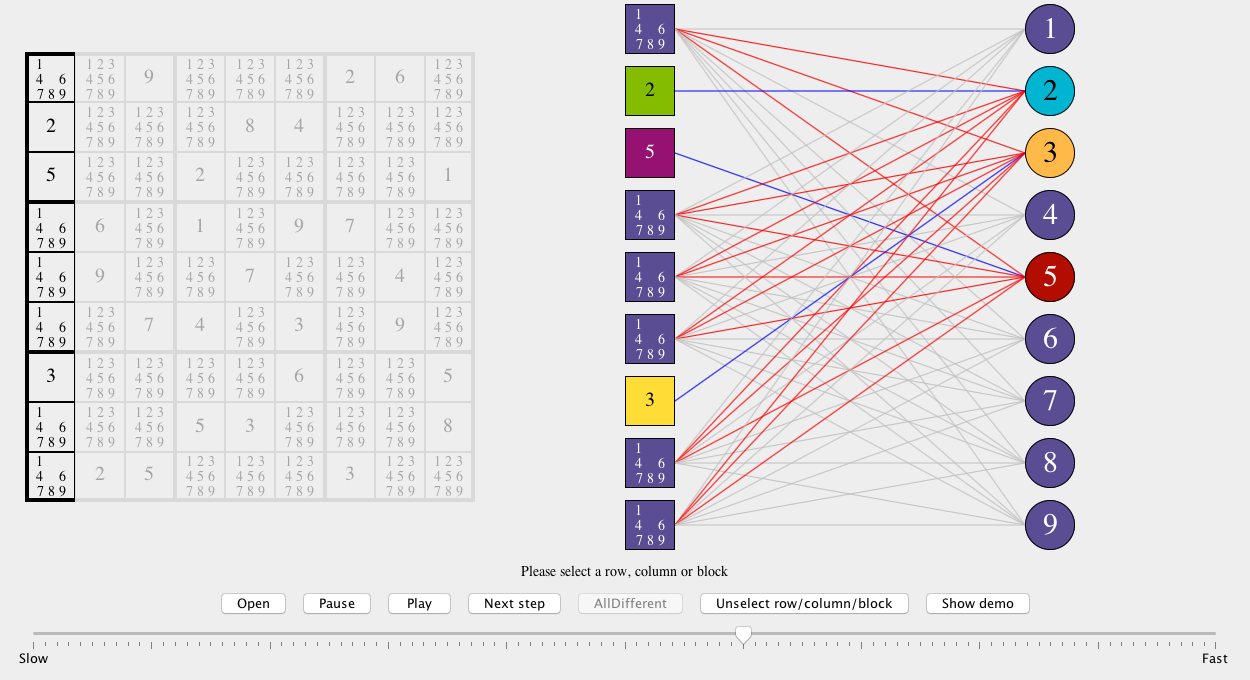
\includegraphics[width=8cm]{images/proof_of_concept/1.png}}
\hfill
\subfigure[5th row after running the all-different algorithm]{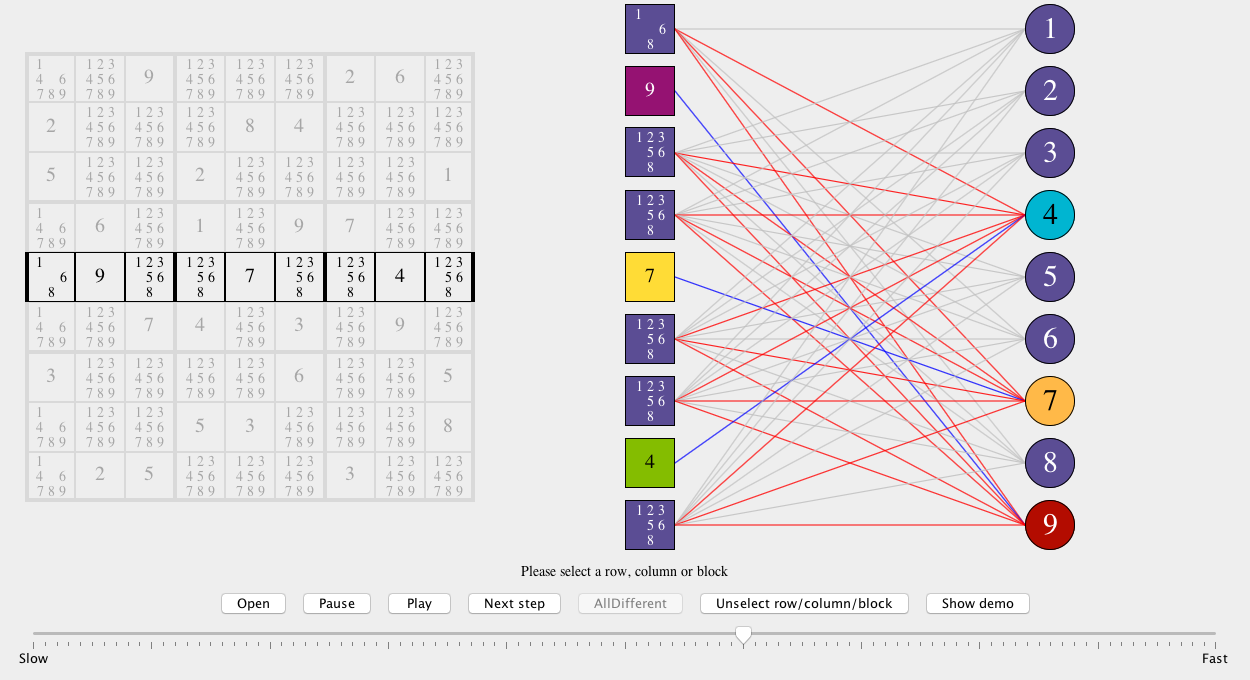
\includegraphics[width=8cm]{images/proof_of_concept/2.png}}
\vspace*{2cm}
\hfill
%\caption{Title for both}
%\end{figure}

%\begin{figure}[h]
\hfill
\subfigure[6th row after running the all-different algorithm]{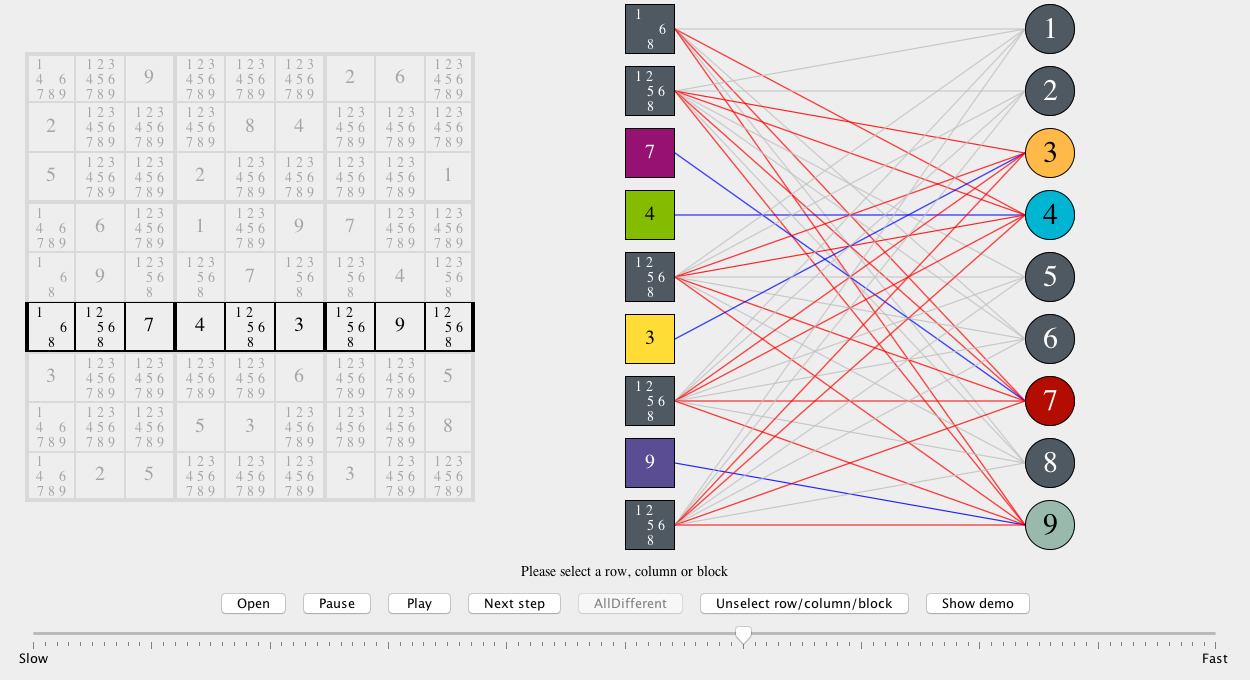
\includegraphics[width=8cm]{images/proof_of_concept/3.png}}
\hfill
\subfigure[4th 3x3 sub-grid after running the all-different algorithm]{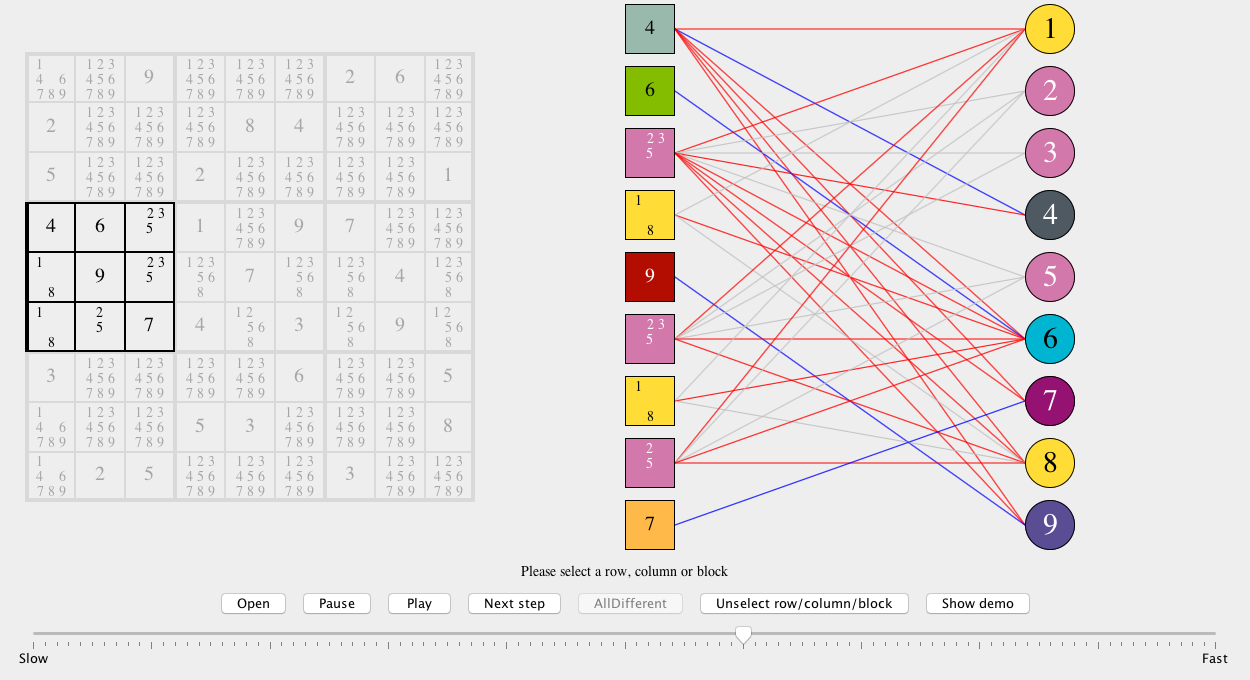
\includegraphics[width=8cm]{images/proof_of_concept/4.png}}
\vspace*{2cm}
\hfill
%\caption{Title for both}
%\end{figure}

%\begin{figure}[h]
\hfill
\subfigure[1st column after running the all-different algorithm]{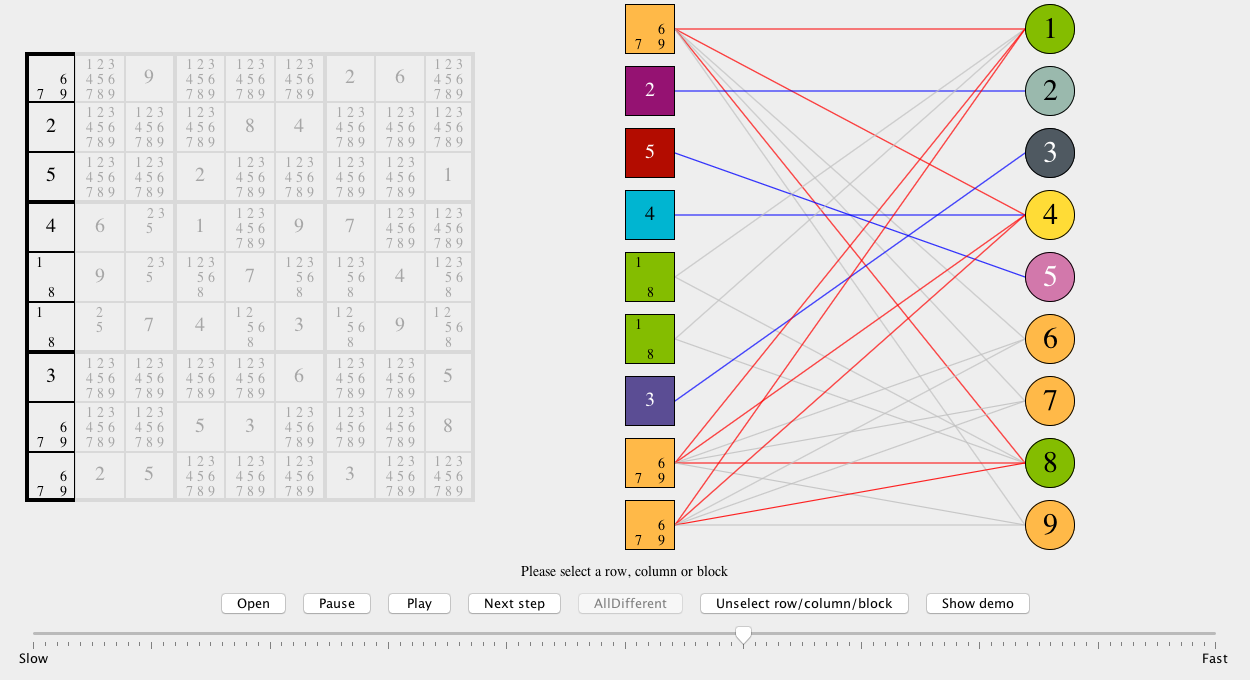
\includegraphics[width=8cm]{images/proof_of_concept/5.png}}
\hfill
%\subfigure[Proof]{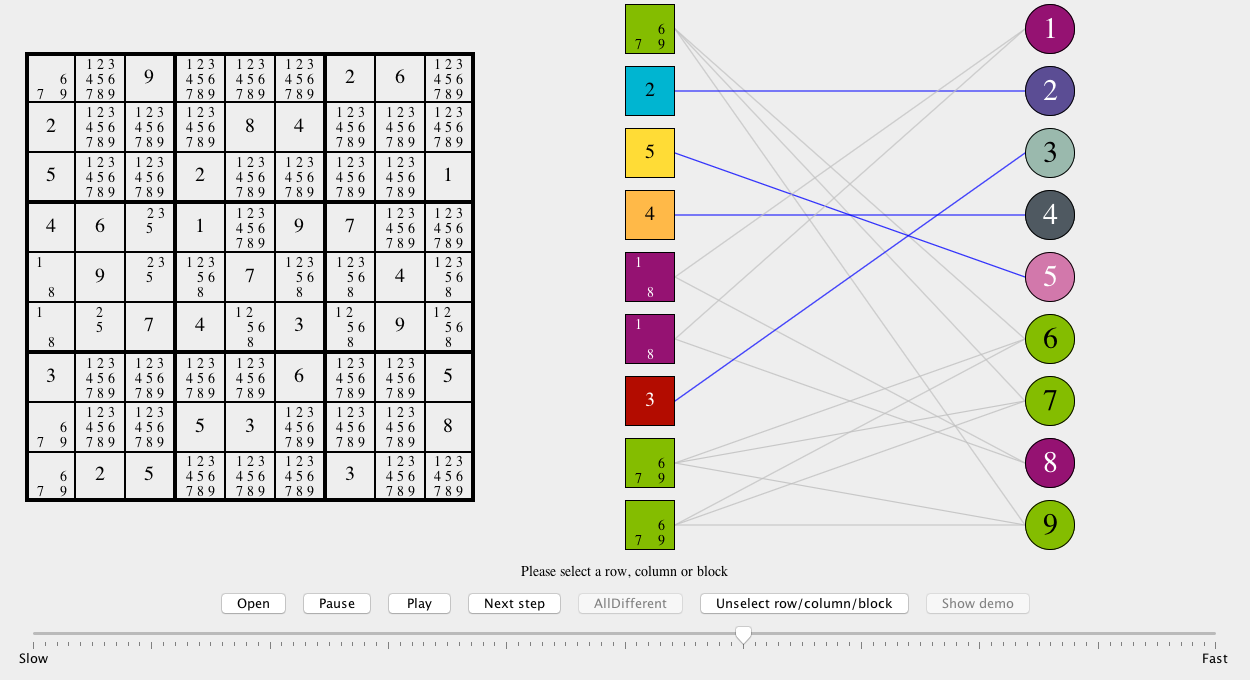
\includegraphics[width=8cm]{images/proof_of_concept/6.png}}
\hfill
\caption{Steps in the demo}
\label{fig:proof_1_5}
\end{figure}

\clearpage 

\begin{figure}[h]
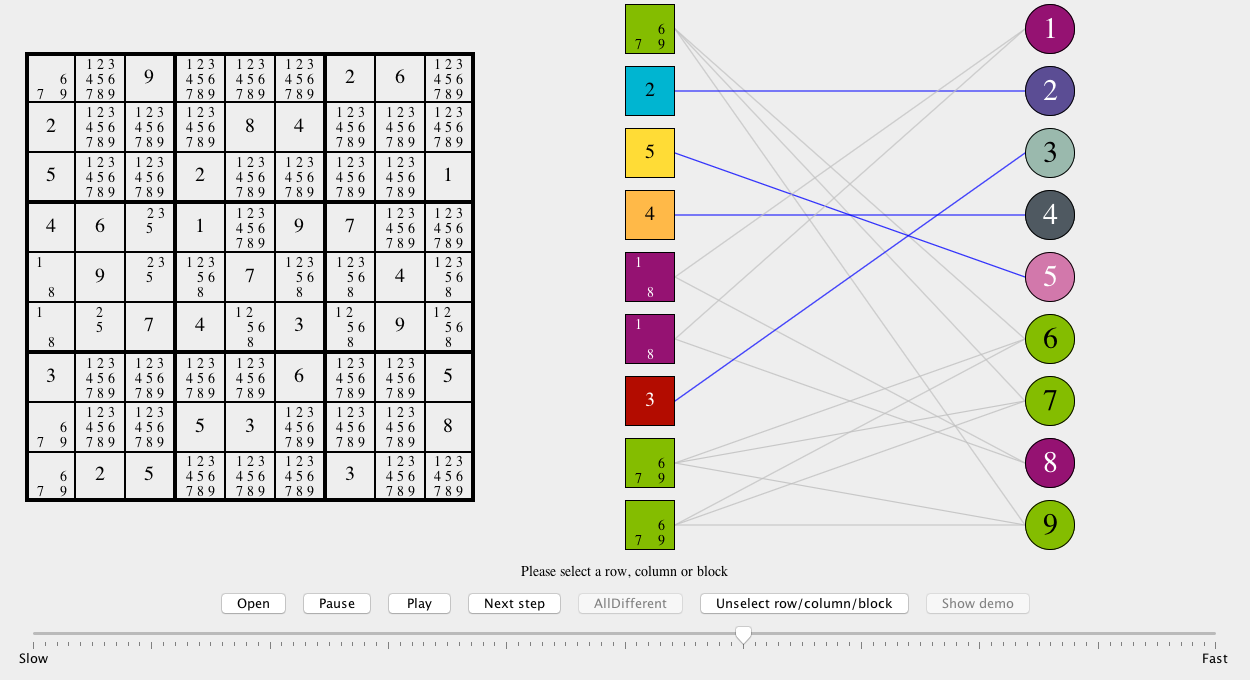
\includegraphics[width=16cm]{images/proof_of_concept/6.png}
\caption{State of the program after running the demo}
\label{fig:proof_6}
\end{figure}

\noindent As seen in ~\Cref{fig:proof_1_5}, the all-different algorithm performs changes only to the selected 9 cells  inside a row, column or 3x3 sub-grid. 

\noindent The end result of following the above steps can be seen in ~\Cref{fig:proof_6}. This state mimics the human thinking when solving a Sudoku. In the 1st column there are two cells with a domain of ${1, 8}$, but we don't know yet which cell will take which digit. What we do know though, is that the digits ${1, 8}$ will be distributed in that two particular cells, therefore in the last step, after running the all-different algorithm on the 1st column we can observe that the digits ${1, 8}$ disappear from the domains of the rest of the cells in the selection.

 
\chapter{Implementation}
\label{chap6implementation}

\noindent The Graphical User Interface (GUI) is inside a JLayeredPane which is a special swing component that allows components inside it to overlap according to their specified depth. In my implementation, the backmost layer contains a JPanel responsible for the drawn edges in the graph. The layer above contains the rest of the GUI represented by the Sudoku puzzle on the left hand side of the screen, and the vertices of the graph on the right hand side of the screen. By using a layered panel, the edges of the graph can be drawn behind the vertices.

\noindent The Sudoku Grid present on the left hand side of the screen is made up of 9 by 9 Sudoku Cells positioned at specific locations. When a new Sudoku Cell instance in made, its ith row and jth column number are passed as arguments to the constructor. Using the information related to its location in the grid, it is now possible to render the border of each cell. Initially all the top, left, bottom and right borders have a width of 1px. To represent the 3 by 3 sub-grids, specific borders are set to have a width of 2px. In the end, the 9 by 9 grid is given an overall thick border by specifying a width of 4px to the cells that are in the first and last columns and rows. All Sudoku Cells contain a JLabel with text retrieved from the Model denoting which possible values are still available for that particular cell.

\noindent Not visible to the human eye, a new Sudoku grid instance is drawn on top of the existing one, this time with all borders set to a width of 1px. The Sudoku Cells inside this second grid contain the same information about the state of the puzzle retrieved from the Model. Additional information such as a custom background will be applied to these cells as the algorithm progresses. Cells inside the second grid become visible once the user makes a selection. Once visible, the cells inside the selection are animated into their position inside the graph on the right hand side of the screen. When the user performs deselects his choice, the nice cells are animated back into their original position in the grid and become invisible again.
 
\noindent Particular attention was given to make the software thread safe. It is crucial that the application logic doesn’t make the Graphical User Interface unresponsive. To achieve this, the program will run on two threads, one main thread responsible with all the processing need to be done by the program, and the Event Dispatching Thread. 

\noindent The Event Dispatching Thread (EDT) is a background thread used to invoke Swing methods that change the GUI and listen to events associated to components. Most Swing components are not thread safe, therefore bugs such as race conditions could unexpectedly arise if it was to perform the actions from normal threads. The EDT acts as a queue of events that are performed sequentially.

\noindent Throughout the application, Timer objects are used to schedule repeated actions such as the fading out of the components or movement of the cells. The model contains a two-dimensional ArrayList of Timer objects that acts as a queue of animations. Timers on the same level start running at the same time until they all finish. Once all the timers on a level finish, the next level in the two-dimensional ArrayList is started, allowing us to queue a movement of a row after all the cells finish fading out.

%\lstset{language=Java}

%\begin{figure}
%\lstset{caption={Implementation of Tarjan's algorithm %for finding strongly connected %components},label=codeTarjan}
%\lstinputlisting{Tarjan.java}
%\end{figure}

\chapter{Conclusion and Future Work}
\label{chap7conclusion}
``It is one thing to have an algorithm that is theoretically good. It is another to have an algorithm that is simple enough that someone would want to program it and use it in practice.'' \cite{tarjanart}

\begin{figure}[H]
\centering
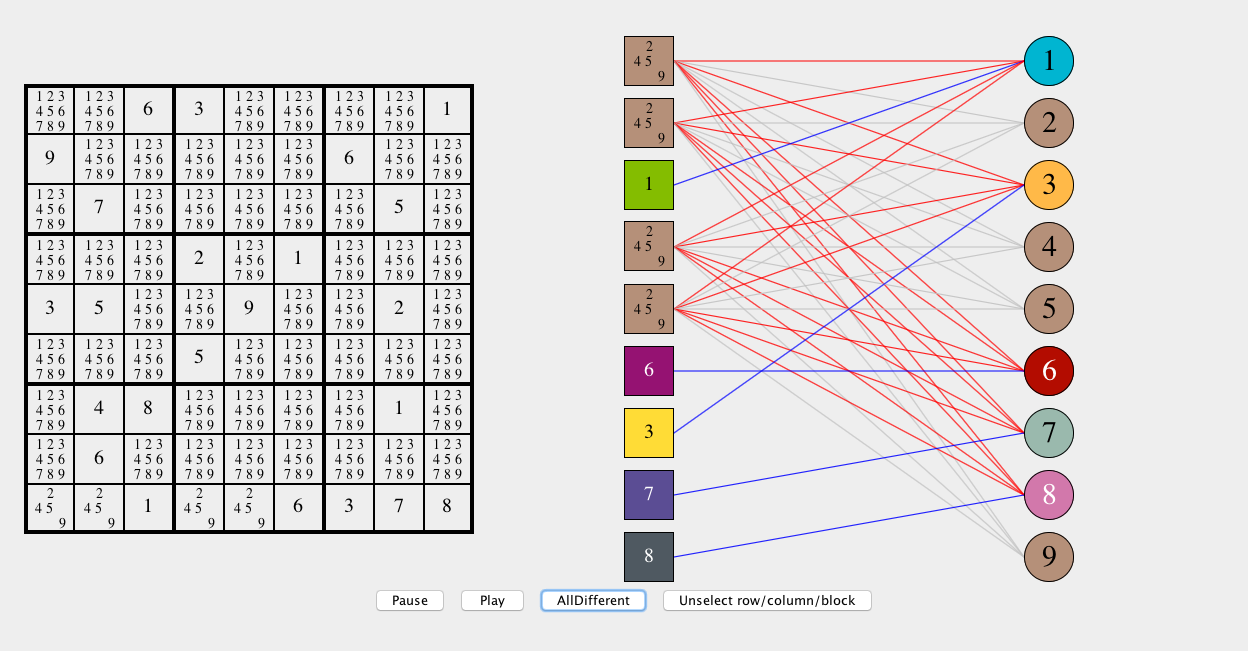
\includegraphics[width=13.2cm]{screenshot.png}
\caption{The state of the program after the all-different algorithm finishes on a row, in this case, the last one.}
\end{figure}

Move this from here
%%%%%%%%%%%%%%%%
%              %
%  APPENDICES  %
%              %
%%%%%%%%%%%%%%%%
\begin{appendices}
\chapter{Running the Program}
Running the program from the command line is done after compiling the source code as follows:
\begin{verbatim}
      > javac *.java
      > java Sudoku
\end{verbatim}
This will open the application loaded with the Sudoku puzzle $\textit{/puzzles/lockedset.txt}$.

\noindent Detailed debug output in the console can be activated using:
\begin{verbatim}
      > java Sudoku debug
\end{verbatim}

\noindent NOTE that the Choco3 library found in $\textit{lib/choco-solver-3.3.1-with-dependencies.jar}$ has to be added to the CLASSPATH environment variable as follows:

\begin{verbatim}
      > export CLASSPATH=$CLASSPATH:/path/to/the/lib/choco-solver-3.3.1-
with-dependencies.jar
\end{verbatim}


\chapter{Proof of concept}

The following sequence of steps will provide a visual proof of the all-different algorithm. The following figures capture the user running the all-different algorithm on 5 predetermined rows, columns or 3x3 sub-grids. For demonstration purposes, the Sudoku instance used is $/puzzles/lockedset.txt$.

\noindent The sequence is as follows:
\begin{verbatim}
      > Open lockedset.txt Sudoku instance
      >
      > Select the 1st column
      > Run the all-different algorithm
      > Deselect the column
      >
      > Select the 5th row
      > Run the all-different algorithm
      > Deselect the row
      >
      > Select the 6th row
      > Run the all-different algorithm
      > Deselect the row
      >
      > Select the 4th 3x3 sub-grid
      > Run the all-different algorithm
      > Deselect the sub-grid
      >
      > Select the 1st column
      > Run the all-different algorithm
      > Deselect the 1st column
\end{verbatim}

\noindent Alternatively, the user can press the $Show Demo$ button to run the same steps.

\noindent Detailed description about why the last state of the program is a proof that the algorithm works as expected is provided in Chapter~\ref{chap5alldiffdemo}.
\end{appendices}

%%%%%%%%%%%%%%%%%%%%
%   BIBLIOGRAPHY   %
%%%%%%%%%%%%%%%%%%%%

%\bibliographystyle{plain}
%\bibliography{mybib}
\printbibliography

\end{document}
